%%%%%%%%%%%%%%%%%%%%%%%%%%%%%%%%%%%%%%%%%%%%%%%%%%%%%%%%%%%%%%%%%%%%%%%%%%
%%%%%                         CHAPITRE 1                            %%%%%%
%%%%%%%%%%%%%%%%%%%%%%%%%%%%%%%%%%%%%%%%%%%%%%%%%%%%%%%%%%%%%%%%%%%%%%%%%%

\lhead[\fancyplain{}{\leftmark}]%Pour les pages paires \bfseries
      {\fancyplain{}{}} %Pour les pages impaires
\chead[\fancyplain{}{}]%
      {\fancyplain{}{}}
\rhead[\fancyplain{}{}]%Pour les pages paires 
      {\fancyplain{}{\rightmark}}%Pour les pages impaires \bfseries
\lfoot[\fancyplain{}{}]%
      {\fancyplain{}{}}
\cfoot[\fancyplain{}{\thepage}]%\bfseries
      {\fancyplain{}{\thepage}} %\bfseries
\rfoot[\fancyplain{}{}]%
     {\fancyplain{}{\scriptsize}}


%%%%%%%%%%%%%%%%%%%%%%%%%%%%%%%%%%%%%%%%%%%%%%%%%%%%%%%%%%%%%%%%%%%%%%%%%%
%%%%%                      Start part here                          %%%%%%
%%%%%%%%%%%%%%%%%%%%%%%%%%%%%%%%%%%%%%%%%%%%%%%%%%%%%%%%%%%%%%%%%%%%%%%%%%

\chapter{Contexte industriel et objectifs de recherche}
\label{ch:objectives}

%==============================================================================	Résumé du chapitre

\begin{center}
\rule{0.7\linewidth}{.5pt}
\begin{minipage}{0.7\linewidth}
\smallskip

\textit{Dans ce premier chapitre, nous positionnons notre travail par rapport à l'état de l'art de l'existant, en injection-moulage des thermoplastiques. Nous identifions des démarches qui permettent d'améliorer la modélisation du procédé. Enfin, nous identifions les verrous au déploiement du contrôle de la qualité à cent pourcent, ainsi que nos objectifs de recherche pour les lever.
}

%\smallskip
\end{minipage}
\smallskip
\rule{0.7\linewidth}{.5pt}
\end{center}

\minitoc
\newpage

\FloatBarrier
\section{Maîtrise du procédé d'injection-moulage des thermoplastiques}
Dans cette section, nous réalisons une synthèse des techniques employées dans l'industrie afin de maîtriser la variabilité du procédé d'injection-moulage.
Il s'agit dans un premier temps d'effectuer des mesures pertinentes sur l'état du procédé, puis de les analyser afin de pouvoir proposer une modification des réglages adaptée.

% Relecture Éric
% Présenter les contraintes du procédé d'injection
% -> Réglage initial du point de fonctionnement difficle
% -> Peu de dérive du procédé, causes exceptionnelles de Shewart
% -> Pas ou peu de mesure de la qualité en ligne de production, pourquoi ? -> introduire notre travail

\FloatBarrier
\subsection{Cartographie bibliographique}
Notre étude bibliographique \citetitle{nagorny_injection_2017} \cite{nagorny_injection_2017} nous permet de proposer un graphe relationnel à partir des mots-clés associés à 421 publications, de 1970 à 2015, Figure \ref{fig:cartographie}.
% TODO: mettre en valeur son intérêt pour la thèse

\begin{figure}[hbtp]
	\centering
	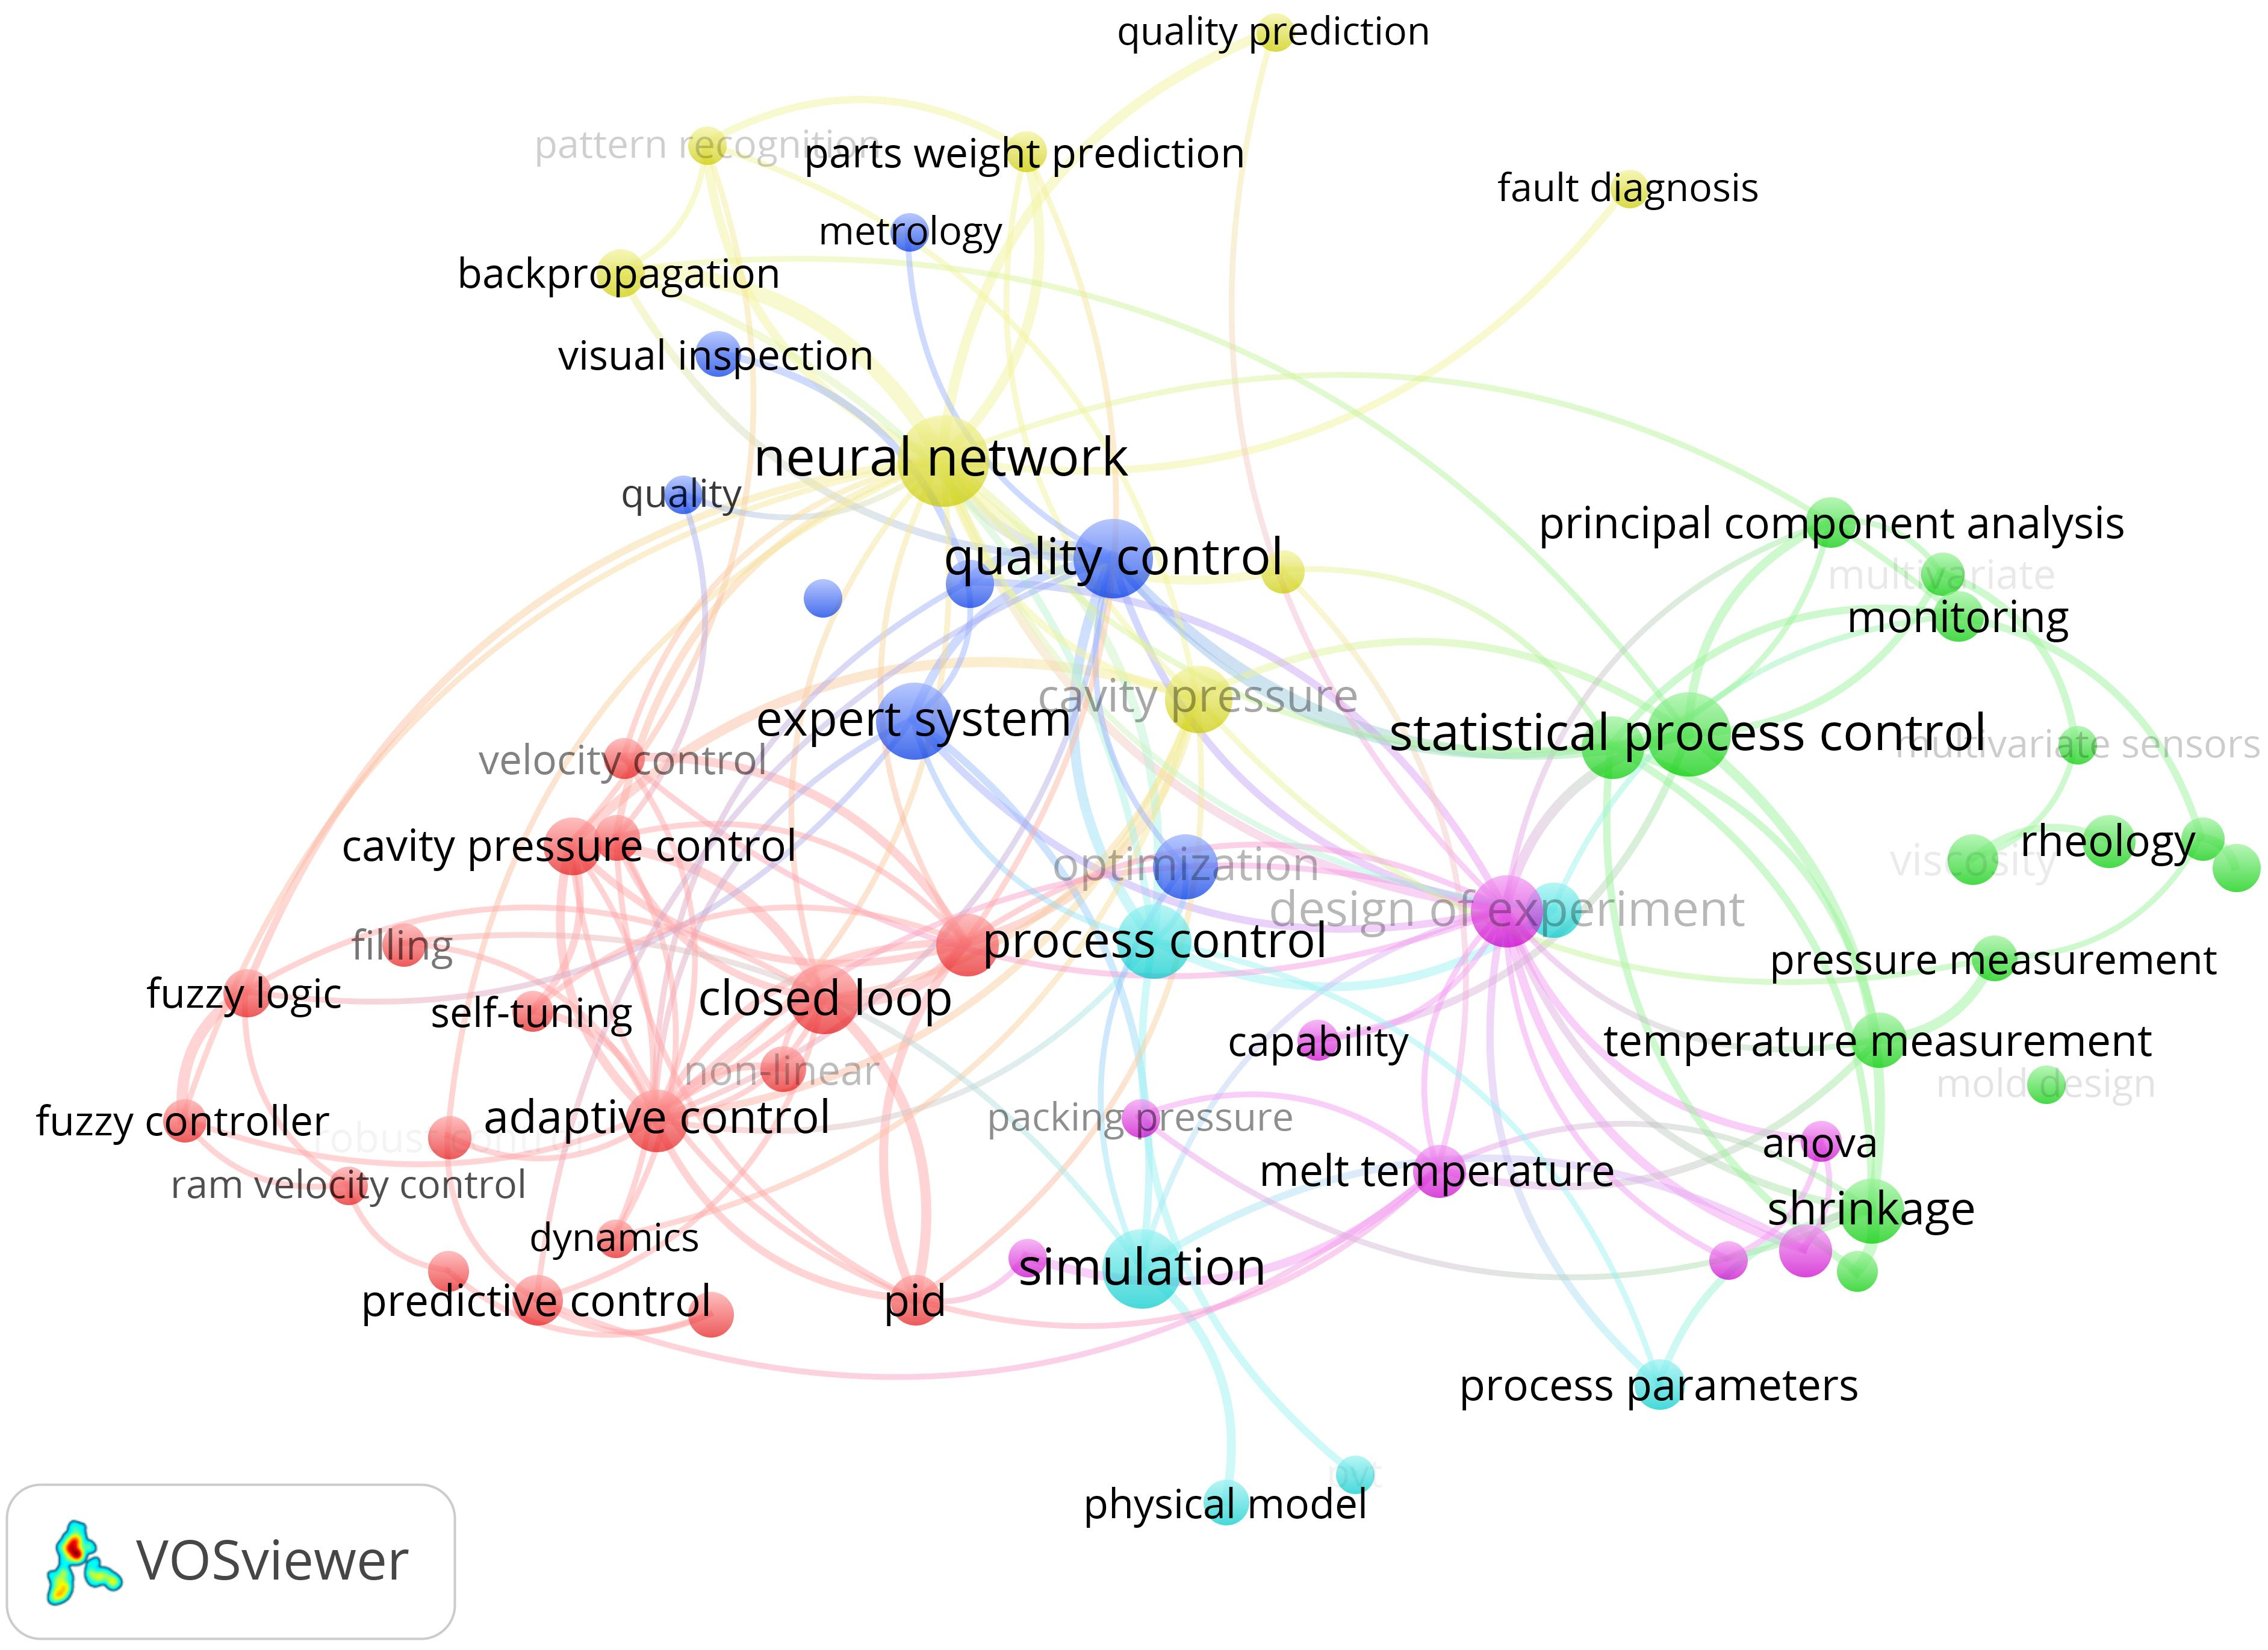
\includegraphics[width=\textwidth,height=\textheight,keepaspectratio]{../Chap1/Figures/tagMapFinalPubliOccurence.jpg}
	\caption{Cartographie bibliographique de la maîtrise du procédé d'injection-moulage.}
	\label{fig:cartographie}
\end{figure}
% TODO: exploiter cette figure

Les mots-clés sont retenus pour l’affichage s’ils apparaissent plus de quatre fois.
Ils sont regroupés par liens communs.
Nous utilisons le formalisme \textit{VOS} (\textit{Visualization Of Similarities}) proposé par \citeauthor{vaneck_vos_2006}, pour modéliser notre base bibliographique \cite{vaneck_vos_2006, van_eck_comparison_2010}.
Nous identifions des axes de recherches importants :
\begin{itemize}
	\item la modélisation physique et la simulation du procédé (couleur cyan),
	\item la régulation du point de fonctionnement par la théorie du contrôle (couleur rouge),
	\item l’analyse statistique (couleur verte),
	\item l’apport des systèmes experts pour régler (couleur bleue),
	\item l’apport des systèmes à réseaux des neurones (couleur jaune).
\end{itemize}

L'analyse statistique est utilisée pour détecter les défaillances du procédé.
Elle s’appuie sur la mesure \textit{in-situ} de variables du procédé, parmi lesquelles les plus utilisées sont la température et la pression.
Les réseaux de neurones sont souvent utilisés pour prédire les caractéristiques des pièces.
Les caractéristiques de qualités du produit, comme la masse ou les dimensions, sont calculées par les réseaux à partir de la mesure de la pression dans le moule.
La littérature propose de réguler les paramètres du procédé d’injection à partir de la prédiction de caractéristiques des pièces.
La prédiction à partir de variables du procédé est préférée à une mesure directe sur la pièce, car la métrologie n’est pas assez développée pour permettre une mesure pièce à pièce en cycle industriel.
À contrario, l'enregistrement des mesures de pression pendant le cycle est très répandue, car elle est implémentée par les fabricants de moules et les fabricants de systèmes de régulations du procédé.
Enfin, nous distinguons (de couleur rouge) les efforts pour la régulation du procédé.
De nombreuses méthodes ont été étudiées et nous remarquons l’intérêt porté aux méthodes adaptatives.
Cependant, chacune de ces méthodes ne s’intéressent qu’à un nombre limité de variables du procédé et des caractéristiques du produit.

%3.3	Commande des transitions de phases
%3.3.1	De la phase d’injection au maintien
%Lors de la transition de la phase d'injection à la phase de maintien, l’asservissement de la machine change (Figure 3). En phase d’injection, c'est la position et la vitesse de la vis ou la pression hydraulique d'injection qui est asservie ({PV3} Figure 6). Cet instant de transition, appelé point de commutation, peut-être spécifié comme une durée, une vitesse de vis ou une position de vis.  Les systèmes de pilotages industriels commerciaux permettent également de définir une valeur de pression maximale mesurée dans le moule qui déclenche la commutation. Cette dernière solution est souvent retenue dans l’industrie. [Kazmer et al., 2010] compare 7 techniques de commande du point de commutation. Il conclue que la température mesurée dans le moule est la plus robuste, et permet de rejeter les variations d’autres paramètres. Le contrôle en position créer une variation des caractéristiques sur les produits deux fois plus élevée qu’un contrôle basé sur la température mesurée dans le moule. Enfin, la commande de commutation par un délai temporel est la moins reproductible avec une variation dix fois supérieure. La commande par pression mesurée dans le moule s'est imposée dans l’industrie car elle permet de garantir la production de pièces complètes sans manque de matière. La pression mesurée n’est néanmoins pas un paramètre indépendant des autres paramètres car elle est fonction de la vitesse et de la température du fondu. L'emplacement des capteurs dans le moule doivent aussi être choisi judicieusement, c’est pourquoi [Garcia et al., 2014] propose de déterminer l’emplacement optimal à partir de l’analyse des mesures obtenues dans des simulations pour de multiples emplacements. Pendant la phase de maintien c'est la pression hydraulique de maintien qui est asservie selon un profil prédéfini ou bien en pression constante car cela garanti un compromis global de qualité des pièces [Chen, 2002].
%3.3.2	De la phase de maintien au refroidissement
%Le canal d’injection relie la buse à l’empreinte. La transition entre maintien et refroidissement doit se faire en fonction de l’état de la matière dans le canal. La solidification de la matière autorise le relâchement de la pression hydraulique et le recul de la vis pour débuter la phase de dosage. La durée de maintien est traditionnellement réglée par un délai temporel préalablement fixé ({PV2} Figure 6). C’est pourquoi [Thomas et al., 1996] développe un capteur de solidification qui permet de piloter le temps de maintien par la détection de la solidification. De même que Chen [Chen, 2002] qui détecte le refroidissement de la matière afin de relâcher la pression de maintien au moment idéal, pour ne pas trop contrainte la matière solidifiée ou en cours de solidification.

\subsection{Modélisation du procédé d'injection-moulage}
Le procédé d'injection-moulage des thermoplastiques est cyclique et séquentiel.
Chaque phase possède des paramètres qui influent de manière non-linéaire sur les phases suivantes et, à terme, sur les caractéristiques du produit fini.
Le moulage par injection est l'étape clé du processus de fabrication des pièces plastiques.
Elle répercute ses défauts sur l'ensemble des étapes suivantes.
Et ce sont les étapes de finitions qui ajoutent le plus de valeur au produit.
Un défaut dans l’une des phases impactera l’ensemble de la chaîne de production et diminuera le rendement global du moyen de production.

\begin{figure}[hbtp]
	\centering
	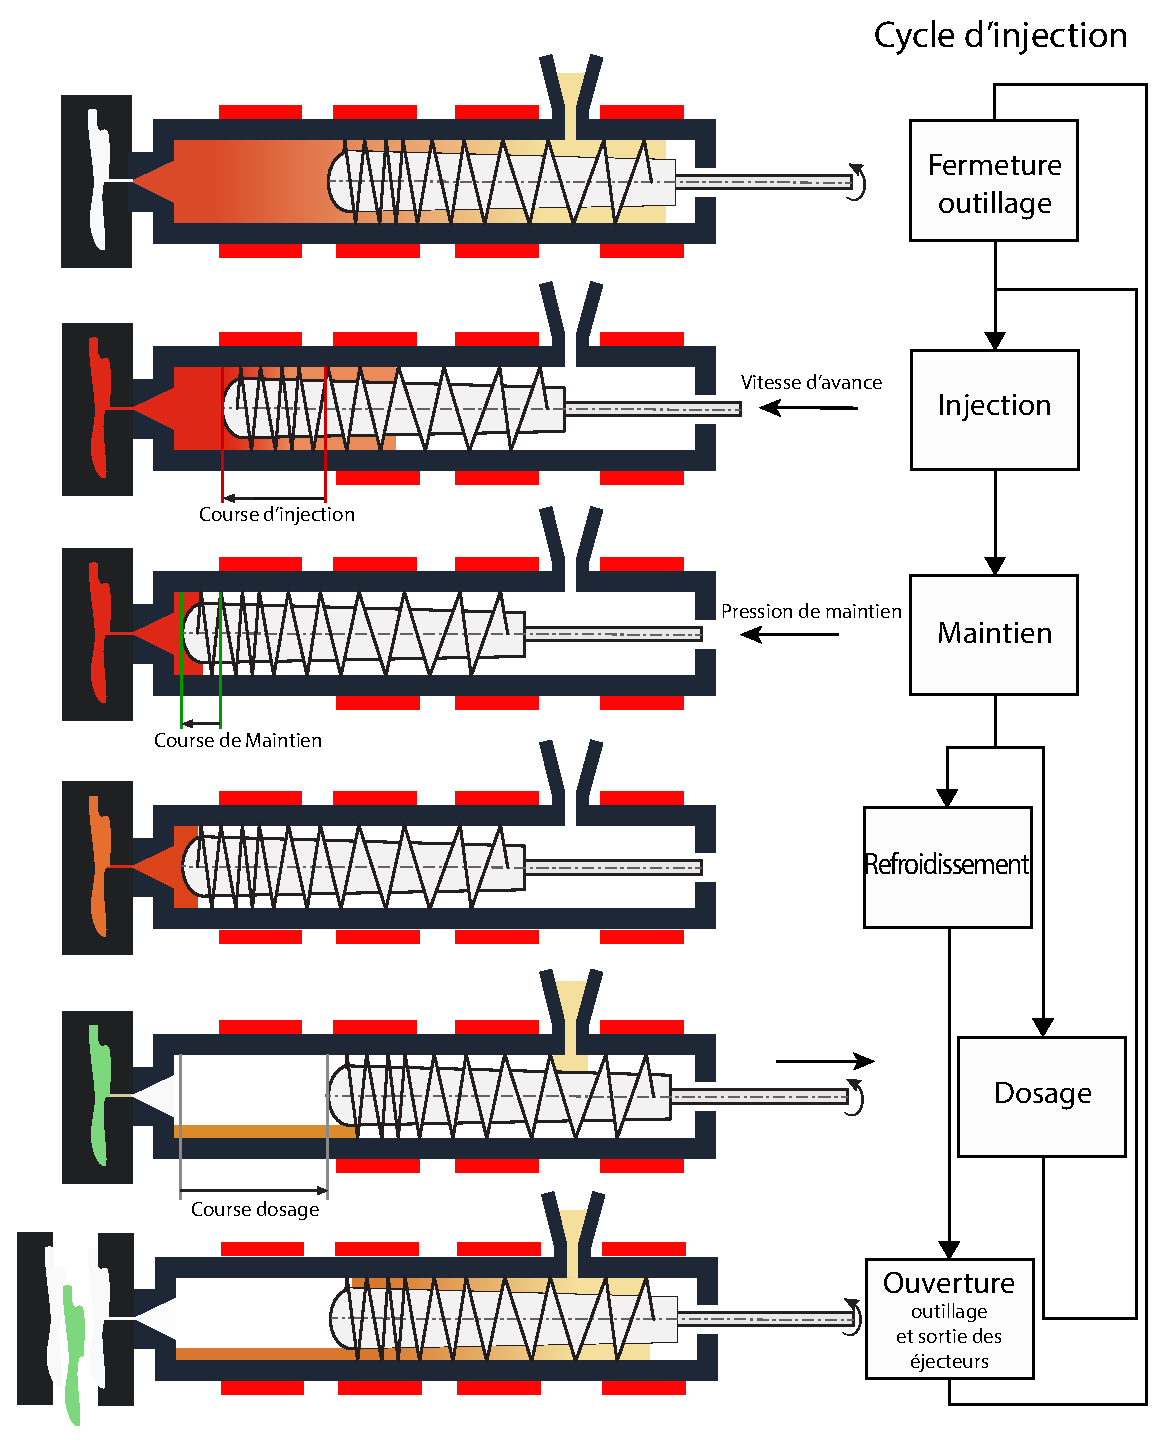
\includegraphics[width=\textwidth,height=\textheight,keepaspectratio]{../Chap1/Figures/SAPRISTI_Schema-cycle.pdf}
	\caption{Schéma-bloc du procédé d'injection-moulage.}
	\label{fig:cycle_injection}
\end{figure}

Afin de mettre en évidence la séquence d’un cycle du procédé, nous proposons un schéma bloc d’un cycle d’injection, Figure \ref{fig:cycle_injection}, dans lequel le dosage est réalisé en parallèle du refroidissement.

\subsubsection{Proposition d'un modèle systémique composé de phases interdépendantes}
Le moulage par injection plastique se décompose en phases interdépendantes, qui conditionnent le produit fini.
\begin{figure}[hbtp]
	\centering
	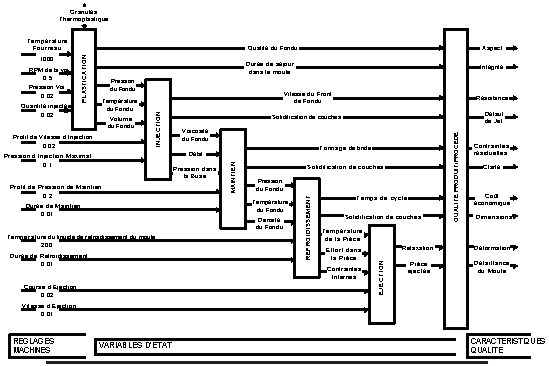
\includegraphics[width=\textwidth,height=\textheight,keepaspectratio]{../Chap1/Figures/Kazmer_1999-Process.pdf}
	\caption{Vue systémique du procédé d'injection-moulage, adaptée de \citeauthor{kazmer_towards_1999} \cite{kazmer_towards_1999}.}
	\label{fig:kazmer_systematic}
\end{figure}
\citeauthor{kazmer_towards_1999} proposent un découpage en cinq phases \cite{kazmer_towards_1999}, Figure \ref{fig:kazmer_systematic}, qui est une  évolution du découpage en trois phases proposé par \citeauthor{ma_design_1974} \cite{ma_design_1974}.
Cette représentation systémique du procédé fait apparaître les variables d’état intermédiaires.
Elle fait également apparaître les relations de dépendance entre les phases, qui sont la cause des caractéristiques du produit.
La dimension temporelle n’est pas prise en compte.
Cela ne permet pas de faire apparaître les opérations qui sont réalisées en parallèles, comme la phase de dosage et la phase d'injection.

\begin{figure}[hbtp]
	\centering
	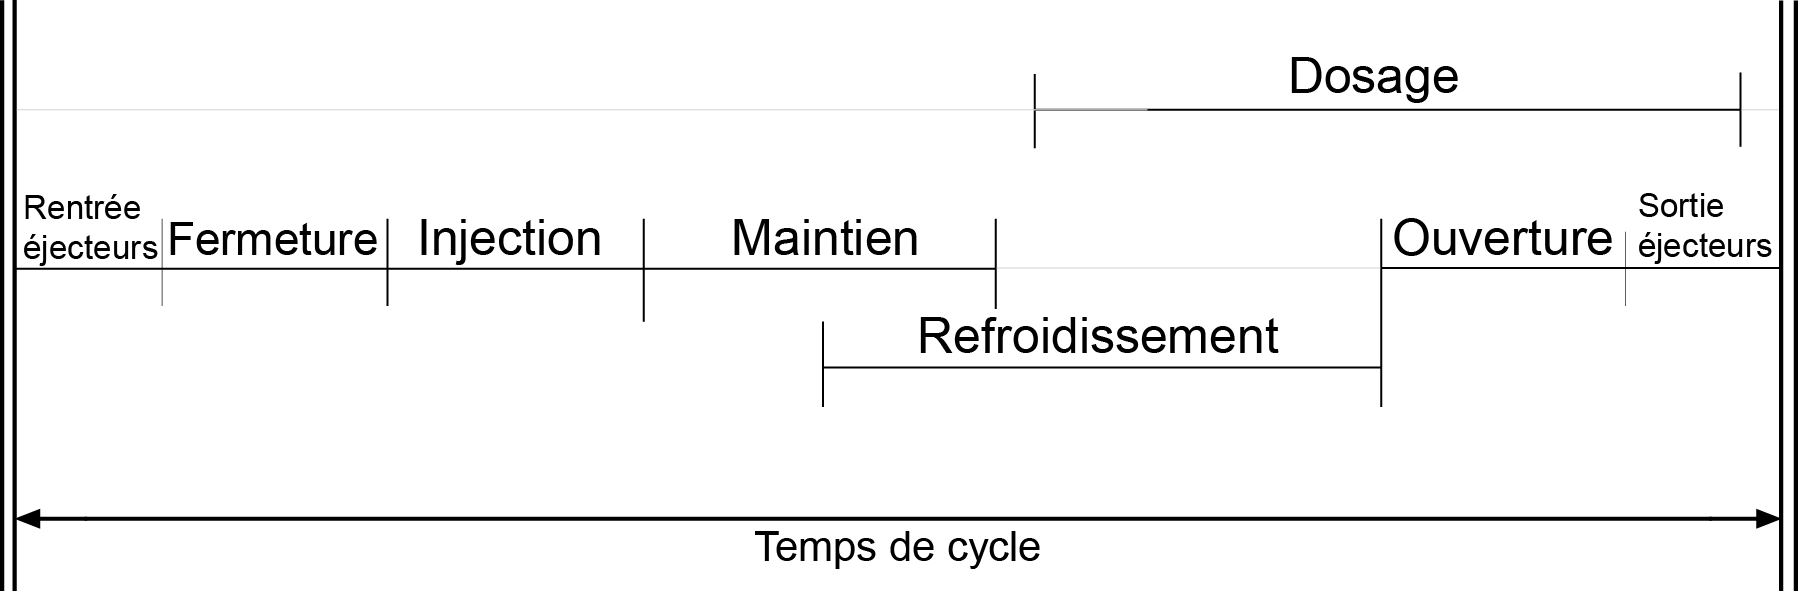
\includegraphics[width=\textwidth,height=\textheight,keepaspectratio]{../Chap1/Figures/SAPRISTI_Chronogramme-Simple.png}
	\caption{Chronogramme du cycle d'injection-moulage.}
	\label{fig:chronogramme}
\end{figure}

Nous proposons d’ajouter la dimension temporelle avec un chronogramme du cycle d’injection, Figure \ref{fig:chronogramme}.
Ce dernier prend en compte les relations temporelles contiguës et parallèles des différentes phases.
On distingue les phases principales d’injection, de maintien et de refroidissement.
La phase de dosage est réalisée en temps masqué.
Elle peut débuter pendant le refroidissement, dès que le canal d’alimentation est solidifié.
Elle se termine avant le début de la phase d'injection.
\citeauthor{thyregod_modelling_2001} définit le temps de refroidissement comme facteur principal de la qualité et de la durée du temps de cycle, pour une production multi-empreintes \cite{thyregod_modelling_2001}.
Il propose ainsi d'optimiser le ratio entre durée de la phase de refroidissement et profit économique réalisé par heure.
Ce critère permet d'optimiser qualité et productivité.
L’objectif est de réduire la durée des phases du cycle.
La durée incompressible de la phase de dosage, réalisée en temps masqué, est la limite à cette optimisation.
Les systèmes de canaux chauds (\textit{hot runner}) réduisent les durées d’injection et de refroidissement : les canaux de distribution de la matière sont maintenus à température par des éléments chauffants de sorte que la matière reste à l’état fondu dans les canaux pendant l’ensemble du cycle.
Enfin, des moules à refroidissement actif, capable de dissiper rapidement la chaleur, réduisent la durée du refroidissement \cite{kazmer_towards_1999}.

\begin{figure}[hbtp]
	\centering
	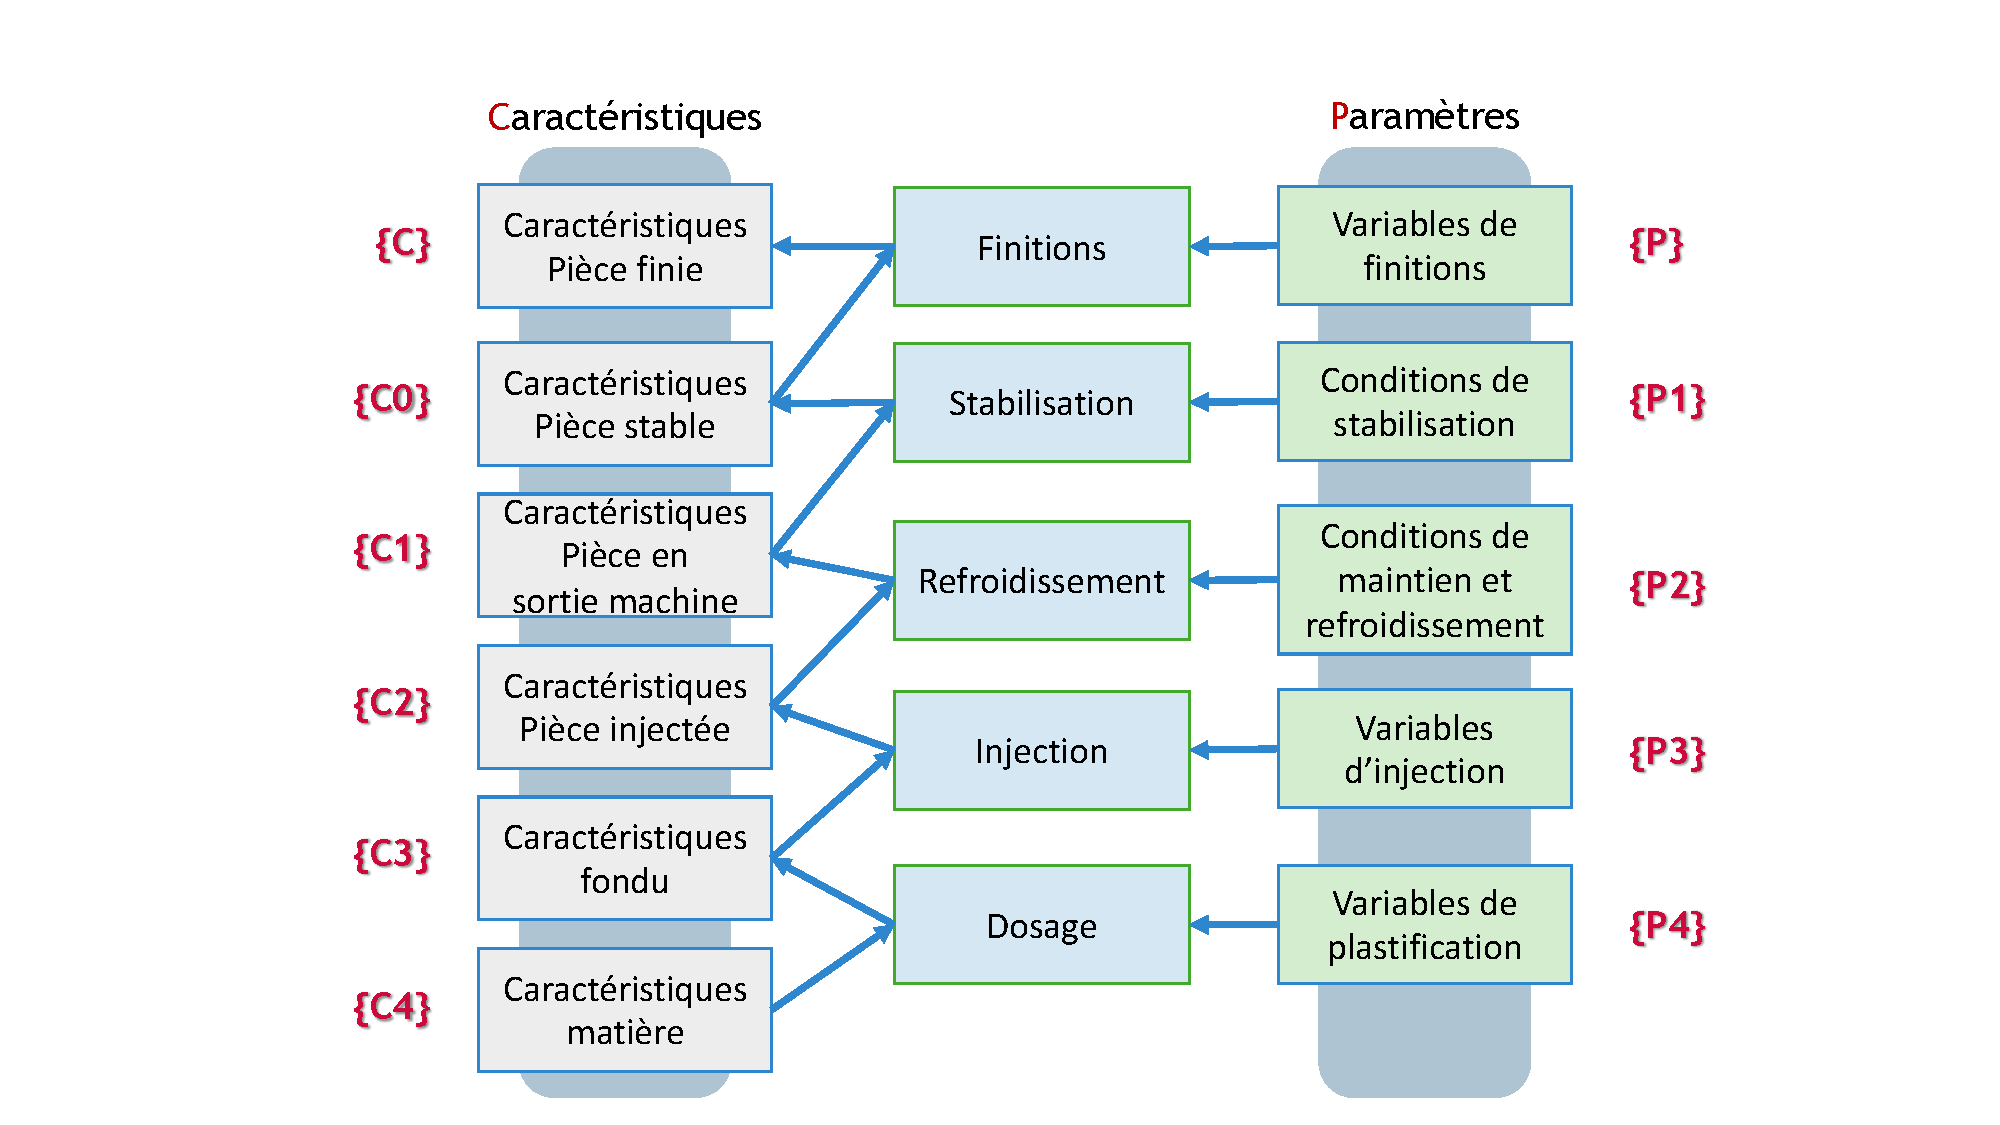
\includegraphics[width=\textwidth,height=\textheight,keepaspectratio]{../Chap1/Figures/Sapristi_ZigZag.pdf}
	\caption{Représentation Zig Zag du procédé d'injection-moulage.}
	\label{fig:zigzag}
\end{figure}

Nous proposons de découper le procédé en cinq phases successives.
Nous proposons une représentation Zig Zag, Figure \ref{fig:zigzag}, qui est complémentaire du schéma-bloc précédent.
La représentation Zig Zag est proposée par \citeauthor{suh_principles_1990} dans sa méthodologie \textit{Axiomatic Design} \cite{suh_principles_1990}.
À la différence de la vue systémique de la Figure \ref{fig:kazmer_systematic}, la représentation Zig Zag fait apparaître les enjeux du procédé : les variables du procédé $\boldsymbol{P_i}$ et les caractéristiques du produit lors de chacune des phases $\boldsymbol{C_i}$.
Les caractéristiques du produit fini $\boldsymbol{C_i}$ sont fonctions de l’ensemble des phases.
De plus, chaque phase est fonction des phases précédentes et des variables du procédé.
Si un réglage est modifié au niveau de l’une des étapes, les caractéristiques du procédé pour toutes les étapes suivantes seront modifiées.
Dans la suite de notre présentation des méthodes de pilotage, nous indiquerons à quelle étape de notre représentation correspond les études citées.

\subsubsection{Revue bibliographique de la modélisation du procédé d'injection-moulage}
En 1987, dans un État de l’Art du pilotage des procédés d’injection-moulage, \citeauthor{agrawal_injection-molding_1987} estiment que de futurs travaux devront réaliser un modèle multivarié du procédé d'injection-moulage, afin de prendre en compte l’ensemble des variables \cite{agrawal_injection-molding_1987}.
Pourtant, aucun des modèles proposés dans la littérature ne prend en compte l'ensemble des variables de ce procédé.
La nature séquentielle et cyclique du procédé rend difficile la réalisation de cette démarche.

\paragraph{Modélisations théoriques du procédé d'injection-moulage}\mbox{} \\
Ces modèles doivent prendre en compte des interactions multi-physiques.
La connaissance de la physique des polymères reste un champs de recherche ouvert.
Le lecteur intéressé par les avancées de la modélisation cristallographique et micro-mécaniques des polymères, en injection-moulage, pourra se référer à la monographie de \citeauthor{galeski_nano_2009} \cite{galeski_nano_2009}.
Les auteurs discutent des contraintes thermo-mécaniques qui s'exercent sur la matière pendant un cycle de production.
Ils analysent les conséquences de ces contraintes sur les propriétés cristallographiques et sur les propriétés mécaniques des pièces.

En 1978, \citeauthor{shankar_dynamic_1978} a le premier développé un modèle non linéaire en temps discret, pour optimiser la vitesse d'avance de la vis et le débit d'injection, dans le but d’obtenir une pièce aux caractéristiques définies \cite{shankar_dynamic_1978}.
À la suite de ce travail, \citeauthor{shankar_mathematical_1982} ont proposé un modèle similaire de l'ensemble du procédé \cite{shankar_mathematical_1982}.
Le modèle est validé par une comparaison entre des simulations et des essais expérimentaux.
\citeauthor{chiu_dynamic_1991} analysent les profils de pression dans le moule, ce qui leur permet de proposer un modèle dynamique du procédé \cite{chiu_dynamic_1991}.
Huit variables d’état sont utilisées : délai avant le début du dosage, pression d’arrivée de la matière pour le dosage ($\boldsymbol{C_3, P_4}$ §\ref{fig:zigzag}), pression d’injection, position de la vis, pression de la vis, volume du polymère dans l’empreinte et débit du polymère ($\boldsymbol{C_2, P_3}$).
En 2000, \citeauthor{delaunay_nature_2000} montrent l'influence de l'évolution du contact entre la matière injectée et le moule pendant le cycle d'injection \cite{delaunay_nature_2000}.
Les précédents travaux assument que le contact entre le moule et la matière est parfait et que les températures à l'interface des deux phases sont identiques.
Or une différence de plus de 20°C est cependant mesurée ($\boldsymbol{C_2, P_3}$).
À partir d'une mesure invasive par un capteur de température dans l'outillage, ce travail identifie un modèle qui prend en compte l'évolution du contact d'un point de vue thermique.
Les auteurs concluent sur la difficulté d'identification de leur modèle, lorsque d'autres paramètres du procédé sont modifiés.
Les limites de la modélisation mathématique du procédé d'injection-moulage sont les hypothèses fortes qui sont faites en amont.
\citeauthor{bereaux_series_2004} proposent un modèle de l'étape de plastification ($\boldsymbol{P_4}$ §\ref{fig:zigzag}) \cite{bereaux_series_2004}.
À partir des lois d'écoulement non-newtoniennes et de transformation de la matière, \citeauthor{moguedet_use_2009} proposent un modèle par simulation en éléments finis \cite{moguedet_use_2009}.
Ces simulations sont coûteuses en ressources de calculs et en temps.
Leurs utilisations pour ajuster les réglages nécessite que le résultat soit obtenu pendant la durée du temps de cycle du procédé.
Malgré les puissances de calculs aujourd’hui disponibles, cette durée
est toujours incompatible.
Les simulations éléments-finis sont en revanche indispensables pour la conception des pièces et des outillages, car elles permettent le dimensionnement des structures.
Elles permettent également d’optimiser les conceptions \cite{gao_adaptive_2008}.

Dans la suite de nos travaux, nous ne nous appuierons pas sur la connaissance des modèles physiques.
Nous utiliserons une démarche empirique pour modéliser le procédé.
Nous nous intéresserons en particulier à la modélisation des caractéristiques des pièces produites, pour des paramètres du procédé données.

\paragraph{Modélisation empirique par plan d'expérience}\mbox{} \\
Les plans d’expériences permettent de construire un modèle polynomiale approximé d’un système à plusieurs paramètres.
Ils permettent d'adapter la quantité d’essais expérimentaux à réaliser en fonction de l'ordre du modèle que l'on cherche à obtenir.
Les essais sont réalisés suivant une table de variation des paramètres.
Nous discutons des plans d'expériences dans le Chapitre 3 §\ref{subsec:doe}.
Le modèle obtenu permet d'optimiser une sortie en fonction des paramètres, et ainsi de trouver un point de fonctionnement idéal.
En 1994, \citeauthor{blyskal_applying_1994} utilisent les plans d’expériences afin de déterminer les paramètres optimaux pour produire des dimensions de pièces cibles \cite{blyskal_applying_1994}.
De nombreux travaux utiliseront par la suite cette démarche.
En 2013, \citeauthor{fei_practical_2013} réalisent une étude rétrospective de l’utilisation des méthodes de Taguchi en injection-moulage des thermoplastiques \cite{fei_practical_2013}.
Ils distinguent deux utilisations faites dans la littérature : produire un jeu de données de mesures, pour ensuite construire un modèle par réseaux de neurones (nous réaliserons cette démarche dans le Chapitre 3 §\ref{sec:dataset}) ; optimiser la conception d’une pièce et de son outillage en simulation numérique.

\paragraph{Modélisation empirique par réseaux de neurones}\mbox{} \\
L'utilisation des réseaux de neurones dans les systèmes industriels est proposée dès 1980.
Le procédé d'injection plastique possède des paramètres interdépendants et non-linéaires.
Par leur construction, les réseaux de neurones sont des fonctions non-linéaires adaptées à ces problèmes aux multiples entrées.
Nous détaillons les algorithmes à réseaux de neurones dans le Chapitre \ref{ch:metric_learning} §\ref{parag:neural_networks}.
En 2000, \citeauthor{schnerr-haselbarth_automation_2000} proposent le système \textit{Intelligent Quality Control} \cite{schnerr-haselbarth_automation_2000}.
Un algorithme à réseaux de neurones est utilisé pour prédire la qualité des pièces produites à partir des variables du procédé.
Les données d’apprentissage proviennent d’un plan factoriel à trois niveaux, sur trois paramètres du procédé : température du fondu, pression de maintien et vitesse d’injection ($\boldsymbol{P_4, P_3, P_2}$ §\ref{fig:zigzag}).
150 points de mesures de la pression dans le moule ($\boldsymbol{C_2, C_0}$ §\ref{fig:zigzag}) sont enregistrés pendant les phases d’injection et de maintien.
La masse de la pièce est mesurée avec une précision de 1 milligramme et la plage d’essai couvre une variation de masse de 1,4\%.
Le réseau est alors capable de prédire la masse des pièces avec une exactitude de 86 à 95,2\%, soit une moyenne de 7 milligramme d’erreur sur la masse.
Ces résultats mettent en valeur l'intérêt des modèles qui utilisent des réseaux de neurones.
Enfin, dans sa thèse, \citeauthor{chen_characteristics_2002} proposent une méthodologie pour établir le profil de vitesse d’injection ($\boldsymbol{P_3}$ §\ref{fig:zigzag}) \cite{chen_characteristics_2002}.
Il modélise l’avancée du front du fondu à l'aide de réseaux de neurones.
Il conclut sur la nécessité de garantir une vitesse de front constante lors de l'injection, afin d’obtenir une qualité produit optimale.
Il modélise également la température du fondu par réseau de neurones, et obtient un profil de température à imposer pour la plastification ($\boldsymbol{P_2}$ §\ref{fig:zigzag}).

\subsection{Vers le pilotage du point de fonctionnement : Étude bibliographique}
Nous réalisons une synthèse de notre étude bibliographique \citetitle{nagorny_injection_2017} \cite{nagorny_injection_2017}.
L'historique des avancées réalisées pour la maîtrise du procédé d'injection-moulage montre une évolution vers le pilotage cycle après cycle des paramètres du procédé.
L'objectif du pilotage est d'optimiser le procédé afin d'obtenir la meilleur qualité possible pour le produit.
\begin{figure}[hbtp]
	\centering
	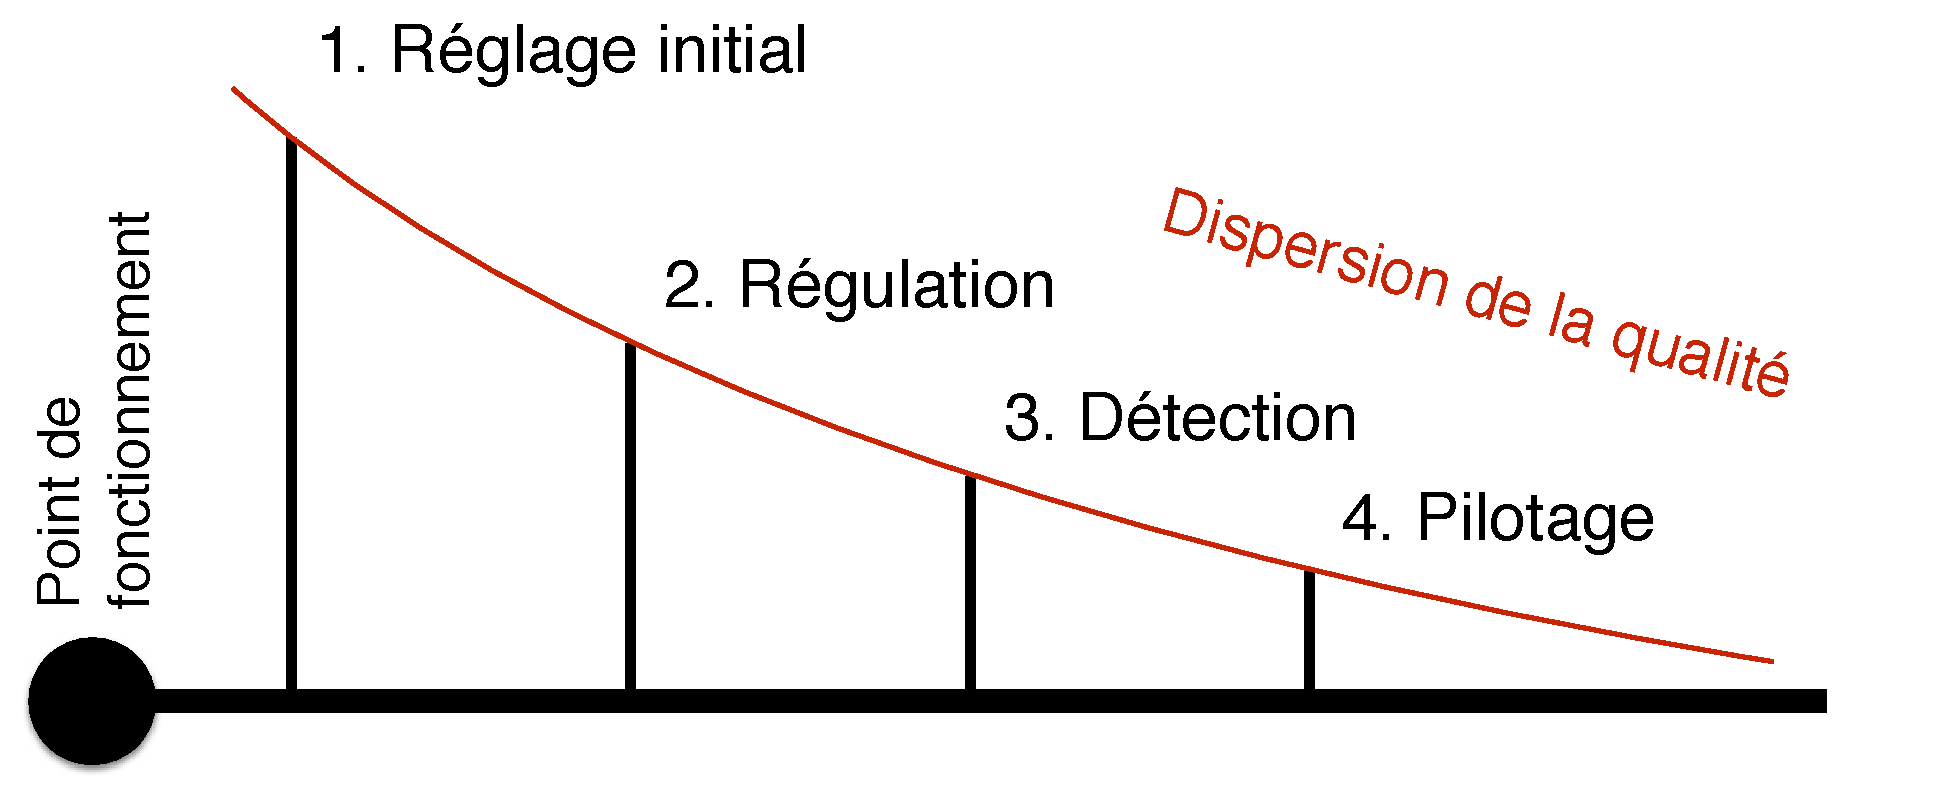
\includegraphics[width=\textwidth,height=\textheight,keepaspectratio]{../Chap1/Figures/Sapristi_EtatArt_Pilotage_en_Injection_Plastique.pdf}
	\caption{Vers le pilotage du point de fonctionnement du procédé pour optimiser la qualité du produit.}
	\label{fig:vers_le_pilotage}
\end{figure}
Réaliser le pilotage du point de fonctionnement nécessite la maîtrise de l'ensemble des étapes précédentes : le réglage initial d'un point de fonctionnement, la régulation de ce point de fonctionnement et la détection de situations hors-contrôles.
La Figure \ref{fig:vers_le_pilotage} récapitule cette démarche.

\subsubsection{Réglage initial du point de fonctionnement}
La pratique industrielle du procédé d'injection-moulage fait appelle au savoir-faire du technicien pour régler le point de fonctionnement initial.
Un point de fonctionnement est associé aux caractéristiques du produit.
De plus, le procédé d'injection-moulage n'est pas bijectif : il existe plusieurs points de fonctionnement pour des caractéristiques de produit identiques.
L’approche classique de réglage employée par le technicien régleur est l’essai-erreur.
Aussi, lors du démarrage du procédé, les premiers cycles de la production sont dédiés au réglage initial.
Des échantillons sont pris quelques secondes après leurs sorties du moule et leurs qualités est rapidement mesurée par observation visuelle.
Dans un premier temps, il s'agit de contrôle l'absence de manque de matière (trous dans la pièce), puis les déformations géométriques importantes et enfin les traces de brûlures et givrages.
L’opérateur utilise ensuite ses connaissances pour améliorer les réglages et respecter le cahier des charges.
Sur les pièces les plus techniques, des mesures géométriques manuelles sont effectuées à l'aide d'un comparateur.

\citeauthor{richard_analyse_2009} analysent les stratégies employées par des techniciens régleurs \cite{richard_analyse_2009}.
Les observations ont été recueillies sur un intervalle de dix années par \citeauthor{pastre_role_2004} \cite{pastre_role_1994, pastre_role_2004} auprès de 13 régleurs d’une entreprise de fabrication de produits, dont la qualité de finition est élevée \cite{pastre_role_1994, pastre_role_2004}.
Leurs niveaux de compétences et leurs parcours professionnels sont variés.
Certains ont une formation technique, mais beaucoup ont appris par la pratique sans formation initiale.
Les résultats de cette étude montrent que la cause principale des différences de réaction entre régleurs \textemdash la dispersion de réglages \textemdash est liée à la difficulté de lecture de la courbe de la pression hydraulique mesurée par la machine.
La forme de cette courbe est utilisée par les techniciens régleurs pour déduire l’état du procédé.
Les causes de défauts sont connues de l’ensemble des régleurs.
Les systèmes d'assistance au réglage proposent d'ajouter des indicateurs de l’état du procédé, ce qui permet d'éviter les difficultés de lecture de la courbe de pression.

\paragraph{Apport des systèmes experts}\mbox{} \\
Les systèmes experts permettent de choisir des couples paramètres-procédés fonctionnels, afin de produire des pièces plus rapidement, lors d'une mise en place d'une production.
Ces systèmes s’appuient sur une base de connaissances : un ensemble de relations causales pondérées, qui a été construit à partir d'une multitude d'essais et qui modélise également des règles empiriques.
Ces systèmes sont complétés et sont validés par des simulations numériques \cite{jan_expert_1992}.
En 1993, \citeauthor{kameoka_development_1993} vérifient que le système expert est capable de proposer des réglages identiques à ceux d’un technicien-régleur de niveau moyen \cite{kameoka_development_1993}.
Des systèmes hybrides peuvent être constitués de règles empiriques et de cas d'applications spécifiques \cite{shelesh-nezhad_intelligent_1997}.
Ces systèmes simulent une démarche de réglage humaine basée sur la connaissance de relations linéaires simples entre les paramètres du procédé.
\citeauthor{bozdana_development_2002} proposent une base de connaissances de 623 presses à injecter et 27 matériaux différents \cite{bozdana_development_2002}.
Ce système expert permet de sélectionner le couple machine-matériau le plus approprié, pour une pièce donnée.

\subsubsection{Régulation du point de fonctionnement}
Diminuer la dispersion d’un procédé de production permet de limiter les rebuts.
Pour cela, il est nécessaire de maîtriser le procédé.
Il est possible d’asservir les paramètres réglables pour garantir que le procédé reste sur le point de fonctionnement défini.
Cependant, asservir un procédé non linéaire aux multiples commandes et sorties est compliqué.
La littérature de la théorie du contrôle automatique propose de nombreux travaux appliqués aux productions industrielles.
Les recherches aboutissent souvent à des solutions commerciales.
Dans ce domaine d'étude, nous notons le dynamisme du secteur de la chimie de synthèse.
La régulation du procédé s'appuie sur l'analyse de la transformation de la matière, qui change d'état au court du cycle.
Les contraintes qui lui sont appliquées pendant le cycle conditionnent son état final.
Le produit final correspond à la pièce sortie de la machine, après une durée de stabilisation, durant laquelle des modifications géométriques peuvent se produire (par exemple des déformations liées aux contraintes internes qui se relâchent).
Les premiers développements ont porté sur la régulation de paramètre unique.

\paragraph{Utilisation de l'Automatique}\mbox{} \\
Dès 1975, un asservissement est breveté par \citeauthor{laczko_controller_1975}, sous la forme d'une consigne sur la viscosité de la matière \cite{laczko_controller_1975}.
La pression mesurée dans l'outillage permet de réguler la pression hydraulique qui est appliquée pendant le cycle d'injection, afin de garantir une consigne sur la viscosité de la matière.
Cette asservissement est hydraulique et ne nécessite pas de micro-contrôleur.

%\paragraph{Régulation de la pression dans l'outillage}\mbox{} \\
% \citeauthor{maitre_sur_1997} montrent que la position du front du polymère fondu est régi par une équation en pression à double non linéarité \cite{maitre_sur_1997}.
Dans la littérature, la caractéristique du produit la plus étudiée est la masse de la pièce ($\boldsymbol{C_0}$ §\ref{fig:zigzag}).
Le paramètre du procédé qui est le plus étudié pour la régulation est la pression dans l'outillage \cite{fara_evaluation_1985, kamal_dynamics_1987} ($\boldsymbol{P_3}$ §\ref{fig:zigzag}).
Sur ce sujet, \citeauthor{fara_control_1988} évalue l'utilisation des régulateurs PI et PID (\textit{Proportionnel Intégrateur Dérivateur}) \cite{fara_control_1988}.
Dans son travail de doctorat, le système hydraulique du vérin d’injection de la presse est modifié pour inclure deux servovalves, afin de piloter la pression d’injection et d’asservir la pression mesurée directement dans le moule.
% Il obtient une meilleure réponse pour la pression hydraulique par PI, pour la pression dans la buse par PID, et pour la pression dans le moule par PI ou PID.
Les valeurs des correcteurs Proportionnel, Intégrateur et Dérivateur sont choisies à partir de simulations.
Les expérimentations montrent que la valeur de la pression dans l'outillage a un comportement non linéaire.
La régulation est effectuée à l'aide d'un gain échelonné sur la servovalve, selon la valeur de la pression.
Ce procédé de régulation provoque néanmoins des oscillations de pression à la fin de la phase d'injection, car la commande de la valve est binaire.

En 1987, \citeauthor{agrawal_injection-molding_1987} réalisent un état de l'art du contrôle du procédé d’injection-moulage, dans lequel il indique que les régulateurs PI (\textit{Proportionnel Intégrateur}) et PID (\textit{Proportionnel Intégrateur Dérivateur}) sont difficilement utilisables, car il n’existe pas d’état d’équilibre pour l’ensemble de la plage d'états du procédé \cite{agrawal_injection-molding_1987}.
Il conclut sur l’intérêt des contrôleurs autorégulateurs, contrôleurs optimaux et contrôleurs prédictifs.
Ces contrôleurs ne réagissent qu’à une unique variable, mais le procédé à des interactions multivariées.
Les contrôleurs uni-variés entrainent un risque pour la robustesse de la régulation, car ils ne prennent pas en compte les interactions entre les paramètres.
C'est pourquoi, ils peuvent avoir l'effet opposé de celui souhaité.
Le risque est de dérégler un procédé qui est stabilisé.
Le contrôleur uni-varié peut appliquer une correction idéale pour variable, mais cette correction sera erronée pour les autres variables, d'où l'effet opposée qui dérèglera le procédé.
Enfin, \citeauthor{agrawal_injection-molding_1987} argumentent la proposition que les caractéristiques de la matière fondue doivent être mesurées en direct, plutôt que de mesurer des variables de la machines ; ceci permet de limiter les erreurs dû aux mesures indirectes.
C'est le début de la mise en place de capteurs directement au contact de la matière, dans l'outillage.
Nous qualifions ces méthodes de mesure "invasives" pour le procédé.
Elles nécessitent une intégration compliquée au sein de l'outillage.

Par la suite, \citeauthor{fara_comprehensive_1990} développent une régulation de la pression dans le moule qui est capable de rejeter des perturbations externes, tel que la variation des propriétés du polymère et de la matière fondu ($\boldsymbol{P_1}$ et $\boldsymbol{P_2}$ §\ref{fig:zigzag}) \cite{fara_comprehensive_1990}.
Il conclut sur la nécessité d'implémenter un contrôle multivarié et adaptatif.
En 1995, \citeauthor{kazmer_dynamic_1995} proposent le système \textit{Dynamic Feed Control} afin d'équilibrer le débit d'injection de la matière pour les moules multi-empreintes ($\boldsymbol{P_3}$ §\ref{fig:zigzag}) \cite{kazmer_dynamic_1995}.
Plusieurs valves permettent de réguler la pression dans chacune des empreintes, pendant la durée du cycle.
Les résultats obtenus montrent une réduction de 75\% de la variabilité de la masse des pièces produites.
La capabilité long terme (Cpp) du procédé augmente de 0,52 à 1,67.
Ce système demande un développement spécifique de l'outillage du moule.

Des travaux s'intéressent à la régulation de la température de la matière fondue ($\boldsymbol{P_4}$  §\ref{fig:zigzag}), par \citeauthor{kamal_injection_1986} \cite{kamal_injection_1986, gomes_injection_1986}, puis par \citeauthor{gustafson_model_1987} \cite{gustafson_model_1987}.
La vitesse d’avance de la vis lors de l’injection ($\boldsymbol{P_3}$ §\ref{fig:zigzag}) est également régulée par \citeauthor{pandelidis_optimal_1988} \cite{pandelidis_optimal_1988}.
Une boucle de régulation Linéaire Quadratique (commande \textit{LQ}) est conçue et ses paramètres sont identifiés.
Les résultats expérimentaux montrent de meilleures performances qu’avec une régulation PID.
Le temps de réponse aux perturbations est notamment plus rapide.

\paragraph{Apport de la modélisation par réseaux de neurones}\mbox{} \\
Plusieurs travaux proposent de modéliser une partie du procédé d'injection afin de réguler certains paramètres du procédé.
Nous détaillerons la théorie des réseaux de neurones dans le Chapitre \ref{ch:metric_learning} §\ref{parag:neural_networks}.

\citeauthor{demirci_numerical_1997} régule la vitesse d'avancée du front de la matière fondue à partir des mesures de la pression d'injection ($\boldsymbol{P_3}$ §\ref{fig:zigzag}) \cite{demirci_numerical_1997}.
% Le réseau de neurone utilisé est entrainé afin de déterminer la position du front en connaissant la position précédente.
% Cette approche itérative permet de proposer des actions correctives pour garantir une vitesse de front cible.
Dans le même temps, \citeauthor{woll_pattern-based_1997} \cite{woll_pattern-based_1997} propose de réguler deux variables du procédé : la pression d'injection et la température du fourreau ($\boldsymbol{P_3}$, $\boldsymbol{P_2}$ §\ref{fig:zigzag}), afin d'obtenir un profil d'évolution de la pression dans le moule déterminé.
Un réseau de 36 neurones d'entrées, 3 neurones intermédiaires et 2 neurones de sorties est retenu.
Le modèle prend en entrée un échantillonnage de 36 valeurs discrètes du profil de pression et calcule en sortie les dimensions de la pièce qui sera produite.
Le réseau de neurone modélise cette relation à partir d'un jeu de données de 81 profils de pressions.
Ces profils ne sont pas obtenus par expérimentation, mais ils sont simulés par un modèle physique simplifié du procédé.
Le réseau de neurones approxime la simulation qui couteuse en ressource de calcul.
Le réseau propose une réponse sur deux paramètres à partir de 36 variables d’entrées.
Les dimensions des échantillons obtenues expérimentalement avec cette régulation sont mesurées à l’aide un pied à coulisse digital (précision de 10 micromètres), plusieurs jours après la production.
L’utilisation du réseau permet de régler et réguler le procédé afin d’obtenir une longueur d’échantillon voulue.
Les auteurs concluent sur la nécessité d’utiliser un modèle multivarié non linéaire pour modéliser le procédé d’injection.
Les réseaux de neurones sont particulièrement adaptés à cette tâche.

\citeauthor{michaeli_online_2009} régulent la pression dans l'outillage à partir de la consigne de pression du vérin hydraulique d’injection \cite{michaeli_online_2009}.
Un modèle par réseau de neurones dispose d'une base d'apprentissage de 15 cycles d’injection-moulage avec différentes configurations de réglages.
La température de la matière dans le moule est mesurée par capteur infrarouge ($\boldsymbol{C_2}$ Figure 6).
La pression d'injection est régulée ($\boldsymbol{P_3}$ §\ref{fig:zigzag}) afin de suivre le diagramme Pression-Volume-Température, de transformation du matériau pendant l'ensemble du cycle.
Avec la mise en place de cette régulation, les résultats expérimentaux  montrent qu’une augmentation de 20°C de la température de la matière fondu ne cause qu'une augmentation de 0,07\% de la masse de la pièce ; ce qui est négligeable.
En comparaison, la même augmentation, sans la régulation, entraine une diminution de 1.27\% qui n'était pas acceptable.

\paragraph{Apport du contrôle adaptatif}\mbox{} \\
Le contrôle adaptatif\footnote{Le contrôle adaptatif est développé dès 1979 par \citeauthor{landau_adaptive_1979, egardt_stability_1979} \cite{landau_adaptive_1979, egardt_stability_1979}} est expérimenté en injection-moulage dès 1983 par \citeauthor{sanschagrin_process_1983} \cite{sanschagrin_process_1983}.
10 paramètres sont régulés ($\boldsymbol{P_4}$, $\boldsymbol{P_3}$, $\boldsymbol{P_2}$ §\ref{fig:zigzag}) et 3 caractéristiques sont mesurées : masse de la pièce ($\boldsymbol{C_0}$), pression maximale dans la cavité ($\boldsymbol{C_2}$), écartement maximal du moule ($\boldsymbol{C_2}$).
L'algorithme d'identification utilise la méthode des moindres carrés généralisés\footnote{L'algorithme des moindres carrés généralisés qui est utilisé dans le travail \citeauthor{sanschagrin_process_1983} a été initialement implémenté en 1976 par \citeauthor{bethoux_approche_1976} pour l'étude de la fabrication de papiers et de la distillation \cite{bethoux_approche_1976}}.
La température du fourreau ($\boldsymbol{P_4}$ §\ref{fig:zigzag}) n'a pas été prise en compte dans cette étude.
L'auteur justifie cette absence car une modification de la consigne de la température du fourreau est effective après un retard de dix cycles d’injection, à cause de l'inertie thermique de l'outillage.
Trois séries d'essais sont réalisées.
Chaque série d’essais ne s’intéresse qu’à quatre paramètres sur les dix possibles.
Cette démarche peut créer des corrélations statistiques biaisées.
Aussi, il est préférable de réaliser l'analyse de l'ensemble des facteurs lors d'un même essai.
L'essai est réalisé pour des pièces à paroi fine (1 millimètre) et des pièces à paroi épaisse (4 millimètres).
Les variations obtenues montrent qu'il est plus difficile d'obtenir une répétabilité de la masse sur les pièces épaisses.
Le paramètre le plus influent sur les pièces est la pression de maintien.
À la suite des essais, les trois paramètres les plus influents ont été retenus pour implémenter une régulation en boucle fermée.
Suite à la régulation de ces trois paramètres, la masse des pièces varie de 0,4\% à 3,6\% et de 0,1 à 0,3\% sans la régulation ; soit une diminution de la variation proche d’un facteur dix.

Dans ces travaux de doctorat, \citeauthor{devos_contribution_1990} réalise une étude exhaustive des paramètres du procédé qui sont influent sur la qualité géométrique des pièces \cite{devos_contribution_1990}.
Il utilise un correcteur PID pour réguler la pression du vérin d’injection, à partir de la pression mesurée à l'intérieur de l'outillage.
Avec ce système, la variabilité géométrique et la variabilité massique sont diminuées de moitié.
L'étude conclue que la mesure de pression maximale dans l'outillage  ($\boldsymbol{C2}$ §\ref{fig:zigzag}) est une mesure qui peut être choisie comme variable de contrôle du passage de la phase d’injection, à la phase de maintien : c'est le point de "commutation".
Cette démarche est aujourd'hui implémentée chez la plupart des fabricants de systèmes de régulation pour l'injection-moulage.

% À un contrôleur adaptatif, [Srinivasan et al., 1991] ajoute une boucle d'apprentissage composée de termes (q(z) et b(z)) proposées par [Shaw et Srinivasan, 1993], afin de réguler la pression dans le moule.
% Ce système est particulièrement adapté à la régulation de systèmes à cycles périodiques.
% L’étude évalue la faisabilité du système par simulation mais ne se confronte pas à un essai expérimental.
% La pression dans le moule est stabilisée en quatre cycles successifs.
% Les auteurs concluent sur la nécessité de réguler également la température du fondu pour garantir le point de fonctionnement.
% [Gao et al., 1994] proposent un contrôleur pouvant trouver les paramètres de réglages par identification récursive de la fonction de transfert en temps discret du procédé.
% Les paramètres du contrôleur sont obtenus par placement de pôle.
% Ils régulent la pression dans le moule afin de suivre un profil défini.
% Des graphiques présentent la réponse du contrôleur à une modification de la température du fourreau que le contrôleur compense.
% Les qualités du contrôleur ne sont pas évaluées numériquement.
Dans ses travaux de doctorat, \citeauthor{tsoi_fuzzy_1997} compare différents contrôleurs pour réguler la vitesse de l'avance de la vis, à partir de la mesure de la pression dans l'outillage \cite{tsoi_fuzzy_1997}.
Il propose l'utilisation de contrôleurs à logique floue, afin de suivre un profil de vitesse.
La logique floue permet de modéliser sous forme continue des relations empiriques, définies à la manière des systèmes experts.
\citeauthor{huang_fuzzy_2000} \cite{huang_fuzzy_2000} contrôlent la vitesse d’avance de la vis à l'aide d'un contrôleur à logique floue, afin de réguler la pression qui est mesurée dans la buse, pendant les phases d’injection et de maintien ($\boldsymbol{C_3}$ et $\boldsymbol{C_2}$ §\ref{fig:zigzag}).
Les expériences sont compilées dans des graphiques de réponses à une commande de pression définie.
Il n'y a pas d’évaluation numérique.
Les graphiques montrent la réponse satisfaisante du contrôleur à la suite d'un changement d'outillage et à la suite d'un changement de température du fourreau.

La régulation du procédé d'injection est une thématique d'étude riche.
L'utilisation d'une grande variété de contrôleurs uni-varié ou bi-varié a été proposée.
Cependant, la régulation de l'ensemble des variables du procédé n'a jamais été proposée.
Nous posons l'hypothèse que la cause est dû à la complexité de la modélisation du système complet.

\subsubsection{Détection de situations hors-contrôles} \label{subsubsec:spc}
Les variations des caractéristiques produit observées sur des produits peuvent avoir différentes origines.
Selon la terminologie de \citeauthor{shewhart_economic_1930} définit dans \citetitle{shewhart_economic_1930} \cite{shewhart_economic_1930}, l'origine des variations se classent en deux catégories : les causes communes et les causes spéciales.
Les causes communes proviennent de nombreuses sources de perturbations aléatoires.
Elles sont inhérentes au procédé.
Elles entrainent une dispersion selon une loi Normale des caractéristiques des pièces produites.
En revanche, les causes spéciales entrainent des écarts de caractéristiques qui dépassent la dispersion aléatoire.
Les causes spéciales doivent être détectées, puis leurs origines devront être identifiées.
Dès 1997, \citeauthor{sherbelis_methods_1997} proposent de définir une fenêtre acceptable dans laquelle les caractéristiques du procédé doivent se situer \cite{sherbelis_methods_1997}.
Cela permet de prendre en compte la variabilité naturelle du procédé.

En 1991, la \textit{Society of the Plastics Industry} \cite{berins_spi_1991} définit la tolérance dimensionnelle acceptable, en injection-moulage, dans un intervalle de 0,2\% à 0,4\% des dimensions attendues.
En 2010, \citeauthor{kazmer_comparison_2010} étudie différents procédés de régulation \cite{kazmer_comparison_2010}. Il observe, quel que soit la méthode utilisée, une dispersion des dimensions inférieure à 0,3\%.
Il conclut que les tolérances précédemment proposées peuvent être dépassée avec des machines modernes et des stratégies de régulations avancées.
Les tolérances attendues en injection-moulage sont définies par l’Association Française de NORmalisation (AFNOR) \cite{afnor_nf_1987}.
Les tolérances dimensionnelles sont spécifier en pourcentage d'écart.
De plus, elles diffèrent en fonction du matériau plastique employé.
La récente norme ISO20457 (\cite{ISO_20457_2018}) reprend en grande partie cette norme établie par l'AFNOR.
Elle spécifie également la méthode de calcul à employer pour le défaut géométrique de diminution des dimensions après le refroidissement (rétractation, retrait ou \textit{shrinkage}).
La norme définit également les causes externes possibles à la variation des dimensions (météorologie, contraintes mécaniques extérieures), ainsi que les causes liées au procédé (mauvais calcul du retrait, déformation de l'outillage, usure de l'outillage).
Les conditions sont également spécifiées : mesures à réaliser entre 16 et 72 heures après la production, une fois que les pièces ont été stockées à 23°C ± 2°C et 50\% ± 10\% d'hygrométrie.
La normalisation des tolérances permet de connaître l'amplitude à surveiller.
Dans le cadre du FUI SAPRISTI, nous travaillons en particulier sur le contrôle de défauts d'aspect, dont la cause est géométrique (défaut de retassure).
L'ordre de grandeur de ces défauts est de l'ordre de la dizaine de micromètres, pour des pièces de plusieurs mètres.
La tolérance requise pour limiter ces défauts est trois ordres de grandeur plus grande que les tolérances requises dans les normes.

\paragraph{Analyse en Composante Principale}\mbox{} \\
Une presse instrumentée moderne fournit une quantité d’informations conséquente sur ses paramètres propres, de même que sur l’état de la matière.
Ces données sont produites pour chaque cycle.
L’Analyse en Composantes Principales §\ref{subsubsec:ACP} permet de réduire la dimension des données.
Cette méthode est employée par plusieurs travaux en injection-moulage des thermoplastiques.
\citeauthor{lu_stagebased_2004} \cite{lu_stagebased_2004} réalisent une ACP sur des mesures réalisés pendant 60 cycles d'injection, pour 16 variables du procédés ($\boldsymbol{C_0, C_1, C_2}$ §\ref{fig:zigzag}).
Le regroupement des composantes fait apparaître quatre phases distinctes, dont deux phases transitoires.
Cette division correspond bien aux phases du procédé définies dans l'industrie : injection, maintien, refroidissement, plastification.
Une analyse détaillée, phases par phases, montre que les températures du fourreau ne sont pas corrélées avec les autres variables du procédé.
De plus, les variables dominantes, pour chacune des phases, ne sont pas toujours les mêmes.
Enfin, des variables qui ne sont pas importantes sont identifiées.
Trois défaillances sont alors introduits en production : une variation de la composition de la matière, une défaillance du capteur de régulation de la température du fourreau et une défaillance de la valve anti-retour de la buse d’injection.
Ces trois défaillances sont très communs en injection-moulage.
Les trois défaillances sont détectées en temps réel, par un test $T^2$ de \citeauthor{hotelling_analysis_1933} \cite{hotelling_analysis_1933} sur les composantes de l'ACP.
% Le procédé présenté associe la division du procédé en phases et une double surveillance : pour chaque phase, par test T2 de Hotelling et par comparaison de l’erreur-type de prédiction.
% Elle permet de détecter les trois erreurs et de les différencier en temps réel par affichage du graphique des contributions à la dispersion globale de chaque paramètre.

\paragraph{Maîtrise Statistique des Procédés}\mbox{} \label{parag:spc} \\
Les travaux fondateurs de la Maîtrise Statistique des Procédés (MSP), \textit{Statistical Process Control}) sont réalisés dès 1930 \cite{shewhart_economic_1930, shewhart_economic_1931}.
% En 1997, \cite{pillet_optimisation_1997} étudie la méthode de prélèvement à employé dans le cas des outillages qui comportent plusieurs empreintes.
% La mise sous contrôle d'une dimension des pièces est réalisée. 
% Le prélèvement systématique de toutes les empreintes est recommandé.
En 2003, \citeauthor{pillet_maitrise_2003} proposent des principes pour adapter la MSP au procédé d'injection-moulage \cite{pillet_maitrise_2003}.
Le choix des variables à contrôler peut se faire sur les paramètres du procédé et sur les caractéristiques du produit.
Il est recommandé de choisir peu de variables. Celles-ci doivent être les plus caractéristiques possibles des défauts déterminé par le cahier des charges.
Enfin, il est recommandé de choisir des variables faciles à mesurer.
Le procédé d'injection-moulage est capable de produire une pièce toutes les 30 secondes, c'est pourquoi le risque de faux positif est ajusté.
Ce risque est généralement défini à plus ou moins trois fois l'écart-type de la distribution de la valeur surveillée.
Dans le cas de l'injection, cela correspondrait à une fausse alarme toutes les 2,5 heures, soit $0,27\%$ de pièces hors-contrôles.
Cette fréquence est trop élevée, c'est pourquoi les auteurs recommandent d'ajuster le risque à 4,5 fois l'écart-type, soit $0,00068\%$ de pièces hors-contrôles, soit une pièce toutes les 992 heures de production.
Cette démarche diminue drastiquement l'intervalle de tolérance du procédé.
En cas de détection de situation hors-contrôle, il est recommandé d'écarter les pièces concernées.
En cas de répétition de cette situation hors-contrôle sur plusieurs pièces, il est recommandé d'arrêter la machine et de faire intervenir le technicien-régleur.
% TODO:
% Risque \alpha +/- 3 sigma = 0.27\% -> 3 heures
% Risque \alpha +/- 4.5 sigma = 0.00068\%  -> 992,5 heures (x397) \cite{pillet_maitrise_2003}
En 2008, \citeauthor{kazmer_comparison_2008} étudie l'utilisation de la démarche MSP \cite{kazmer_comparison_2008}.
Il évalue séparément la mise sous contrôle statistique des variables de la machine ($\boldsymbol{P1}$, $\boldsymbol{P2}$, $\boldsymbol{P3}$ §\ref{fig:zigzag}) et la mise sous contrôle statistique des variables mesurées dans l'outillage ($\boldsymbol{C1}$ et $\boldsymbol{C2}$).
Les paramètres du procédé sont perturbés suivant un plan d'expériences §\ref{subsec:doe}.
Ce travail montre la pertinence de cette méthode.
Néanmoins, les recommandations de \citeauthor{pillet_maitrise_2003} \cite{pillet_maitrise_2003} ne sont pas prises en comptes : la mise sous contrôle n'est pas réalisé sur les variables les plus pertinentes.
En 2016, \citeauthor{liu_window-based_2016} évaluent un algorithme à fenêtre mobile, afin d’identifier les différentes phases du procédé avant d’appliquer le contrôle MSP \cite{liu_window-based_2016}.
% L’étude compare deux algorithmes de détection de phases.
\citeauthor{zhang_statistical_2016} \cite{zhang_statistical_2016} propose de limiter la surveillance aux seuls paramètres du procédé ($\boldsymbol{P_2}$ §\ref{fig:zigzag}), afin d'éviter d'instrumenter l'outillage.
Il se contraint à utiliser les mesures systèmes de régulation des machines : la pression hydraulique et la position de la vis dans le fourreau.
L’objectif est de prédire les défauts sur la masse des pièces ($\boldsymbol{C_3}$ §\ref{fig:zigzag}).
La méthode proposée atteint 91,48\% de détections de défauts de masse des pièces.
Cette méthode obtient de meilleures performances, en comparaison avec une Analyse en Composante Principale.

\subsubsection{Pilotage des caractéristiques de la pièce produite}
Le pilotage d’un procédé demande dans un premier temps de détecter les situations hors-contrôles.
Dans le cas où le procédé n'est pas dans sa configuration cible, on mesure l’écart entre la situation hors-contrôle et la situation cible.
Puis on ajuste un ou plusieurs paramètres réglables du procédé, afin de se rapprocher de la situation cible.
Plusieurs stratégies de pilotage ont été proposées dans la littérature.
Certaines utilise une modélisation physique simplifié du procédé, d'autres s'appuient sur une base de connaissance préétablie ou utilisent une analyse statistique.
Ces systèmes reposent sur l’instrumentation de la presse et de l'outillage pour mesurer les conditions appliquées au polymère.
L'évaluation des performances de ces stratégies passe par la mesure de dispersions des caractéristiques des produits.
Dans une démarche pragmatique, le pilotage des caractéristiques du produit peut également se réaliser en mesurant directement les caractéristiques des produits ($\boldsymbol{C_1}$ et $\boldsymbol{C_0}$ §\ref{fig:zigzag}).
% C'est l'objectif du projet FUI SAPRISTI.
Dans le cadre de nos travaux, nous mesurerons la qualité des pièces juste après la sortie de l'outillage ($\boldsymbol{C_1}$).

Les essais de modélisation informatique ont émergé avec le développement des valves de décompression à commande électrique \cite{ma_design_1974}.
En 2001, \citeauthor{nwokah_control_2001} synthétisent les avancées réalisées dans le cadre du pilotage du procédé \cite{nwokah_control_2001}.
Ils définissent deux contraintes principales au développement du pilotage :
\begin{itemize}
\item la méconnaissance des relations entre les paramètres d’entrées et les caractéristiques finales du produit ($\boldsymbol{P_i}$ et $\boldsymbol{C_i}$ §\ref{fig:zigzag}),
\item le manque de possibilité d’ajustement des réglages du procédé.
\end{itemize}
Ils argumentent que l’amélioration d’une caractéristique du produit se fera souvent au détriment d’une autre caractéristique, ou bien par l'augmentation des coûts de produit.
Cette contrainte de coût est courante pour les productions industrielles à haute valeur ajoutée.

% \paragraph{Ajustement du procédé à partir des caractéristiques du produit}\mbox{} \\
L’ajustement statistique des procédés (\textit{Statistical Process Adjustement}) est un domaine situé à l’intersection de la régulation automatique et de la Maîtrise Statistique des Procédés.
Ce domaine d'étude étudie les relations entre les paramètres du procédé et les caractéristiques du produit, par une approche statistique.
Un exemple de relations entre les paramètres du procédé d’injection-moulage, qui conditionnent les caractéristiques de la pièce produite, concerne la vitesse d'avance ($\boldsymbol{P_3}$ §\ref{fig:zigzag}).
Celle-ci est liée à la viscosité de la matière ($\boldsymbol{C_3}$) et elle définit le débit d’injection ($\boldsymbol{P_3}$).

Il y a également une influence des paramètres du procédés sur la structure interne de la pièce.
Les travaux de doctorat de \citeauthor{giroud_mesure_2001} étudie l'influence des paramètres du procédé ($\boldsymbol{P_3}$) sur les contraintes internes ($\boldsymbol{C_1}$) \cite{giroud_mesure_2001}.
Le profil de pression appliqué à la pièce pendant la phase d'injection conditionne les contraintes internes résiduelles.
Ces contraintes seront figées dans la pièce par la modification de la forme et de l'orientation des chaînes de polymères.
La relaxation de ces contraintes peut provoquer des déformations géométriques.
C'est une des causes principales du retrait, qui apparait plusieurs heures après la production.

\citeauthor{del_castillo_statistical_2006} réalise une rétrospective des travaux réalisés dans le domaine de l'Ajustement Statistique des Procédés \cite{del_castillo_statistical_2006}.
Il identifie les méthodes de modélisation bayésiennes comme des pistes privilégiées de recherche, par exemple dans leurs applications en contrôle.
Nous présenterons ces méthodes d'optimisations dans le Chapitre \ref{ch:metric_learning} §\ref{subsec:bayesian_opt}.
Il est parfois difficile de mesurer les pièces en sortie de machine.
Les causes sont une durée de la mesure trop longue qui est supérieure au temps de cycle, un coût trop élevé ou simplement une mesure non faisable.
De plus, le manque de spécifications concernant les caractéristiques de la qualité des pièces n’a pas encouragé l’utilisation de la mesure directe.
Excepté pour le dimensionnel, la notion de qualité dans les cahiers des charges sont rarement normalisés.
Elles nécessitent l'interprétation humaine, ce qui est difficile à transmettre à programmer dans une machine (c'est un des objectifs de ce travail, présenté dans le Chapitre \ref{sec:metric_learning}).
Pour remédier à ces limites, de nombreux systèmes ont choisi de prédire les caractéristiques des pièces produites ($\boldsymbol{C_1}$ §\ref{fig:zigzag}) à partir de variables du procédé ($\boldsymbol{P_i}$).
La prédiction obtenue est ensuite utilisée à des fins d’ajustement des réglages pour tendre vers un procédé optimal.

\paragraph{Ajustement du procédé à partir des caractéristiques prédites}\mbox{} \\
En 1993, \citeauthor{haeussler_quality_1993} \cite{haeussler_quality_1993} utilisent un réseau de neurones pour prédire la masse et la longueur des pièces ($\boldsymbol{C_1}$ §\ref{fig:zigzag}), à partir des paramètres du procédé ($\boldsymbol{P_3}$, $\boldsymbol{P_2}$).
% Ils entrainent un réseau 9-21-2 à partir des mesures sur une production de 162 cycles continues.
Le réseau prédit la masse des pièces avec 80\% de justesse et la longueur avec 88,2\% de justesse.
Ces résultats sont comparés avec une régression non-linéaire, qui atteint une justesse de 75\% pour la masse et 79\% pour la longueur.
Cette étude conclut sur la nécessité de l'utilisation d'modèle adaptatif pour un réaliser le pilotage en cycle industriel.
Le modèle prédictif doit être enrichit à partir des mesures, au fur et à mesure des cycles.
Le modèle ne doit pas se limiter à modéliser un jeu de données statique.
Nous reprenons cette idée dans nos travaux, en proposant un modèle de la notion de qualité qui est enrichit au fur et à mesure de la production §\ref{sec:metric_learning}.

En 1996, \citeauthor{woll_online_1996} proposent d'utiliser un réseau de neurones pour prédire la masse des pièces, à partir des profils de pressions mesurées dans l'outillage et dans la buse \cite{woll_online_1996}.
Ce modèle permet d'accepter ou de rebuter la pièce produite par l'analyse de l'écart statistique MSP §\ref{parag:spc}.
Le réseau de neurones est appris comme un modèle inverse du procédé.
Les profils de pressions sont les variables d'entrées ($\boldsymbol{C_2}$, $\boldsymbol{C_1}$ §\ref{fig:zigzag}) et les variables de sorties sont les valeurs des consignes de pression de maintien ou de température du fourreau ($\boldsymbol{P_2, P_1}$).
Les paramètres sont ajustés cycles après cycles en comparant le profil de pression courant, avec le profil cible.
L'analyse MSP est réalisée sur la valeur de pression maximale qui est mesurée dans l'outillage.
Le réseau est appris sur un jeu de données issues de simulations, afin d'éviter de réaliser une longue campagne d'essais.
À contrario, dans nos travaux, nous avons choisi de mesurer des données réelles sur des machines industrielles.
% La convergence du modèle étant observé pour 2000 essais.
L'essai est réalisé pour un unique matériau et la caractéristique cible de la pièce est sa longueur.
% Les résultats montrent la capacité supérieure des réseaux de neurones à prédire les non linéarités comparée à la régression linéaire multiple utilisé par SPC.
% L'exactitude de la prédiction des mesures est augmentée de 10\% et le taux de faux positif est réduit de moitié.
% Le réseau rejette les perturbations.
% L'étude conclue sur la nécessité d'entrainer le réseau sur plusieurs profils dont les températures.

En 2004, dans ces travaux de doctorat, \citeauthor{yang_injection_2004} introduit l'utilisation du contrôle prédictif pour ajuster la vitesse d'avance de la vis lors de l'injection \cite{yang_injection_2004}.
Le contrôleur s'appuie sur la littérature du \textit{Global Process Control} (aussi appelée \textit{Engineering Process Control}) qui consiste à utiliser des régulateurs Proportionnels Intégrateur Dérivateurs pour asservir les caractéristiques du produit.
La masse des pièces est prédite à partir des mesures sur le procédé ($\boldsymbol{C_2, C_1}$ §\ref{fig:zigzag}).
À partir de la prédiction, la vitesse d'injection ($\boldsymbol{P_3}$) est ajusté cycles après cycles.
% Un algorithme d'apprentissage itératif en logique floue compense les temps de réponses long des actionneurs.
Ce travail montre la limite que pose l'utilisation des servovalves pour ajuster les paramètres du procédé.
Les servovalves ont un temps de réponse lent, de l'ordre de la seconde.
Ainsi, il est nécessaire d'anticiper leurs actionnements, notamment lorsqu'il s'agit d'imposer des consignes temporelles précises.
À l'aide de l'ensemble des ces techniques, ce travail montre qu'il est possible de détecter les variations de la masse pendant le cycle, sans nécessité une pesée de la pièce.
Il est également possible d'ajuster les conditions de maintien et de refroidissement en conséquence, afin de compenser les variations prédites.
L'auteur conclut sur la possibilité de piloter d'autres caractéristiques du produits, en utilisant la même démarche.

\paragraph{Ajustement à partir des caractéristiques mesurées sur le produit}\mbox{} \\
Dans l'ensemble de la littérature, la diversité des caractéristiques qualité mesurées sur les pièces est limitée.
La masse est la mesure la plus mesurée, car sa mesure peut facilement être réalisée pendant le cycle d'injection-moulage.
Il suffit de disposer d'un bras robotique préhenseur et d'une balance instrumentée.
Les mesures complémentaires de la qualité des produits sont effectuées après de la production d'un lot, mais non pendant le cycle d'injection.
Il serait intéressant de réaliser une caractérisation complète de la pièce produite, pendant le temps de cycle, afin de pouvoir optimiser les caractéristiques des pièces suivantes, à partir de ces mesures.
La limite à cette démarche est la durée des mesures, qui doit être inférieure au temps de cycle.

En 1998, \citeauthor{fournier_conduite_2006} proposent un ajustement des paramètres du procédé à partir de la mesure de la masse du produit \cite{fournier_conduite_2006}.
Le matériau utilisé est le Poly(Téréphtalate de Butylène).
C'est un semi-cristallin sensible aux phénomènes de retrait.
Le système utilise un modèle physique simplifié du procédé pour réguler les paramètres en boucle fermé.
L'écart entre la masse mesurée et la masse cible est ajouté à la boucle de régulation.
Deux perturbations sont appliquées pendant le cycle : un changement de la matière et un changement de la température dans le fourreau.
Afin de limiter les contraintes internes, les pièces passent par un recuit.
Les mesures des retraits volumiques et de résiliences (chocs Charpy) montrent une dispersion de masse réduite de 24\% avec l'utilisation du correcteur sur la masse.
La dispersion du retrait volumique, mesurée deux jours après la production des pièces, est réduite de moitié, mais l'épaisseur des échantillons augmente.
Après recuit, le retrait volumique est diminué de 12\% par rapport à un procédé non régulé.
La résilience après recuit est quant à elle augmentée de 23\%.
L'étape de recuit peut être assimilé aux étapes de peintures qu'une pièce est susceptible de subir.
Une piste de travail importante est de considérer les caractéristiques des produits finaux ($\boldsymbol{C_0}$ §\ref{fig:zigzag}) pour ajuster le procédé.
Cela nécessite nécessairement l'utilisation d'un modèle prédictif, car la pièce finale sera réalisée plusieurs jours après son moulage.
Les résultats obtenus sont encourageants.
L'étude montre qu'il y a un intérêt à ajuster les paramètres du procédé en fonction des caractéristiques du produit mesurées dès la sortie de la machine ($\boldsymbol{P_1}$).
Nos travaux s'inscrivent dans cette démarche.

La même année, \citeauthor{ivester_automatic_1998} proposent une méthode d'ajustement qui s'appuie sur un modèle du procédé qui est construit au fur et à mesure de la production, à partir de la mesure des caractéristiques et des paramètres \cite{ivester_automatic_1998}.
Ce modèle permet de réaliser une optimisation des caractéristiques en ajustant les paramètres du procédé, par descente de gradient (cette méthode est détaillée dans le Chapitre \ref{ch:metric_learning} \ref{parag:neural_networks}).
% Ainsi, le modèle procédé n’est mis à jour que lorsqu’il ne permet plus d’estimer les changements.
L'étude indique que la caractérisation de la qualité des pièces est réalisée par un opérateur humain.
Dans le cadre de nos travaux, nous chercherons à automatiser ce contrôle.
% Cette méthode d’optimisation des réglages requière que l’opérateur entre les paramètres mesurées ou analyse les mesures dans le cas de caractéristiques d’aspect.
% L’étude conclue sur la viabilité de la méthode et sur l’intérêt d’automatiser la mesure de la qualité des pièces.
Cette méthode est néanmoins dépendante des points de fonctionnement initiaux, qui sont choisis aléatoirement.
C’est pourquoi, \citeauthor{yang_knowledgebased_2000} propose l'ajustement des paramètres du procédé par optimisation d'un modèle qui lie les paramètres avec les caractéristiques du produit, préalablement établi \cite{yang_knowledgebased_2000}.
% C’est un modèle multivarié qui permet de rendre indépendant le système des paramètres initiaux avant optimisation.
C’est ce modèle empirique multivarié qui détermine le point de fonctionnement initial.
% Un algorithme d'apprentissage permet d’optimiser ce modèle pour un produit et une machine.
% L’intérêt du modèle préétablie est de proposer un point de fonctionnement.
% L'apprentissage passe par la comparaison des caractéristiques qualités données par le modèle préétablie et des caractéristiques qualités mesurées sur les pièces.
Par la suite, le modèle initial est ajusté au fur et à mesure de la production.
Les caractéristiques prédites par le modèle sont comparées aux mesures réelles, et le modèle est ajusté pour diminuer l'écart de la prédiction.
% L'étude compare la faisabilité théorique obtenue par simulation et le point de fonctionnement donné par le modèle relationnel KBT, puis le point de fonctionnement obtenu par plan d'expérience central composite.
Une comparaison expérimentale est réalisée entre le système proposé et un point de fonctionnement obtenue par résolution d'un plan d'expériences Central Composite (§\ref{parag:doe_cc}).
7 caractéristiques qualités sont mesurées sur le produit.
5 paramètres sont pilotés sur la machine. % et leurs limites sont connues du modèle.
Le protocole expérimental est détaillé.
Les 20 premières pièces de chaque essai ne sont pas prises en compte, afin de stabiliser le procédé.
Par la suite, 5 pièces sont mesurées 15 à 25 minutes après leur sortie du moule pour que leurs caractéristiques géométriques soient également stabilisées.
Nous pensons que l'amplitude temporelle de 10 minutes est trop grande et qu'elle génère une dispersion des mesures.
En effet, si les pièces sont conservées dans le même atelier de production, alors nous pouvons estimer que leur vitesse de refroidissement est identique, aussi pour une même durée de refroidissement, les caractéristiques seront identiques.
Or cette durée de refroidissement varie ici beaucoup. 
Nous recommandons de mesurer les pièces quelques secondes après la sortie du moule, en maitrisant le délai de mesure, afin de limiter cette dispersion.

Les résultats de l'étude montrent que le plan Central Composite n'inclue qu'un petit espace de la plage de réglage du procédé.
Il est alors difficile de trouver un point de fonctionnement optimal, à partir du modèle issu du plan d’expérience.
L'étude aurait pû positionner les bornes du plan d'expériences aux limites du procédé.
Le système d'apprentissage proposé est capable de trouver un point de fonctionnement satisfaisant en 10 séries d'essais, tandis que le plan Central Composite demande 45 séries d'essais.
Enfin, nous notons que la mesure des caractéristiques qualités du produit est ici facilité car ce sont des disques DVD.
Les mesures ont une résolution élevé puisqu'un micromètre laser mesure un profil sur la surface des disques.
La capabilité du moyen de mesure est excellente.
% Et cette capabilité est ici excellente.
Une bonne capabilité du système de mesures est un pré-requis, pour la caractérisation des pièces, et pour le pilotage du procédé.

En 2001, \citeauthor{lau_neural_2001} propose de réaliser un modèle inverse du procédé, à multiples entrées et multiples sorties, par apprentissage d'un réseau de neurones \cite{lau_neural_2001}. % vérifier les capacités de création  d'un modèle multi entrées-sorties du procédé d'injection par réseau de neurones à propagation inverse.
L’objectif est que le réseau suggère des ajustements des paramètres du procédé pour obtenir une pièce cible aux dimensions spécifiées.
Les caractéristiques dimensionnelles portent sur trois longueurs et l'épaisseur de la pièce.
L'apprentissage du réseau est réalisé sur les mesures récoltés pour 100 pièces, en faisant varier 6 paramètres du procédé : la température du fourreau centrale et la température de l'arrière du fourreau, la vitesse de fermeture de l’outillage, la vitesse d’avance de la vis, la force de fermeture, la durée d'injection, la durée de refroidissement, la vitesse d'avance de la vis lors de l'injection et la pression d'injection.
L'étude mentionne que, malgré la répétition de paramètres identiques, les quatre dimensions étudiées varient entre différentes journées de réalisation des essais.
% Il ne suffit pas de répéter des paramètres
Les valeurs des dimensions attendues sont appliquées en entrée du modèle.
Ce dernier indique en sortie les valeurs du point de fonctionnement permettant de produire une pièce avec ces dimensions.
La démarche du système est alors d'obtenir l'écart entre les paramètres pour les caractéristiques actuelles et pour les caractéristiques cibles, puis d'ajuster les paramètres en soustrayant ces écarts, afin de compenser les variations des caractéristiques pièces.
En connaissant le réglage utilisé pour produire les pièces, l'étude propose de régler les paramètres dans des proportions inverses afin de compenser les variations de pièces.
Cette démarche suppose que les paramètres sont indépendants, ce qui n'est pas le cas pour le procédé d'injection-moulage.
% Néanmoins, après 3 itérations de réglages successifs, le réseau parvient à converger vers une erreur quadratique moyenne (RMS) de 0,07.
% Ce résultat est comparé à une précédente étude des auteurs [Lau et Wong, 1998] qui utilisait un système hybride à logique floue qui convergeait en 3 itérations vers une erreur quadratique moyenne (RMS) de 0,06.
% La méthode proposée est moins performante qu'un système à logique flou et réseaux de neurones mais plus simple à mettre en œuvre.
% De plus, une optimisation de la topologie du réseau de neurones, telle que la recherche en informatique la permet aujourd'hui améliorerait ce résultat.

Récemment, en 2015, \cite{johnston_-line_2015} réalise une étude à l'aide d'un plan d'expériences à 12 facteurs de 15 essais, pendant 30 minutes de production par essais, totalisant 942 cycles d'injection-moulage, soit 60 pièces par essais.
% Il dérive des fonctions de transfert et des composantes principales pour chacune des 46 sorties du procédé.
Pour chaque cycle, une boucle d'optimisation évalue et minimise une contrainte imposée, par un ajustement des paramètres du procédés ($\boldsymbol{P_1, P_2, P_3}$ §\ref{fig:zigzag}).
Le contrôleur qui est proposé est capable de détecter les variations du procédé par comparaison avec un modèle de référence préétabli.
% Le contrôleur ajuste alors les paramètres pour atteindre le modèle de référence.
Un objectif de réduction du temps de cycle est ajouté grâce à une pénalité temporelle dans la fonction à minimiser.
Un double objectif est atteint : le temps de cycle est réduit et la variabilité des dimensions des pièces est réduite.
L'étude conclut qu’une optimisation  multi-paramètres, par exemple sur les caractéristiques dimensionnelles, est possible.

\subsection{La mesure de la qualité du produit : un verrou technologique au pilotage}
Nous concluons cette revue de la littérature par un tableau récapitulatif de l’ensemble des articles cités, Tableau \ref{tab:state_art_compare}).
On observe les travaux initiaux qui utilisent la théorie Automatique pour réguler le procédé.
Par la suite, la modélisation non-linéaire a été perfectionnée par l'utilisation des réseaux de neurones
Dernièrement, les travaux s'appuient sur des démarches de Maîtrise Statistique des Procédés et sur la simulation numérique.
Pour chacune des publications, nous identifions les variables du procédé étudiées selon la représentation Zig Zag, présenté dans la Figure \ref{fig:zigzag}, ainsi que les résultats obtenus.
Le procédé d’injection possède plusieurs phases interdépendantes, mais la littérature ne s’intéresse pas à l’étude de l’ensemble des variables et paramètres du procédé.
De nombreuses études présentées se focalisent sur une unique phase du procédé.
% Il a pourtant été montré que des corrélations entre les paramètres et les différentes phases existent.
Les études de la littérature sont centrées sur les paramètres de la phase d’injection ($\boldsymbol{P_3}$).

\begin{figure}[hbtp]
	\centering
	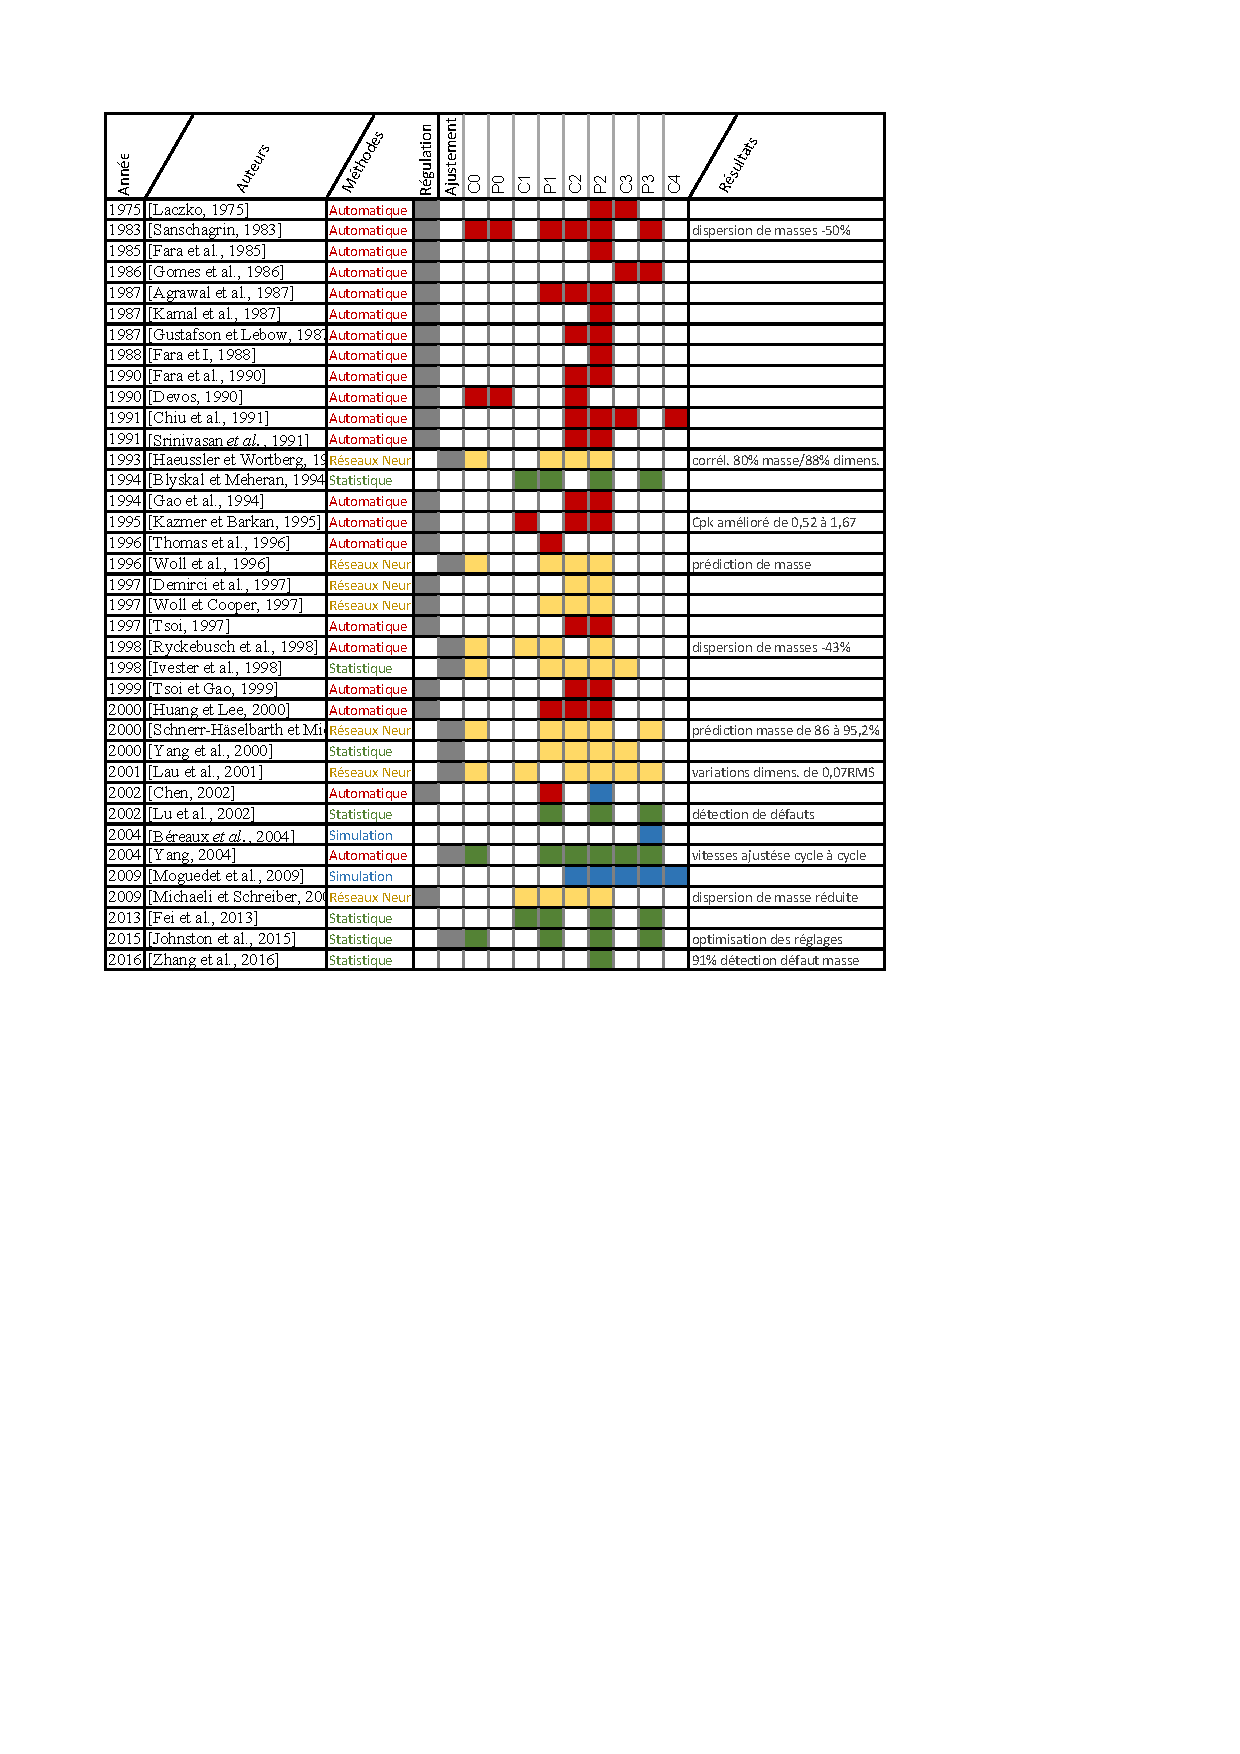
\includegraphics[width=\textwidth,height=\textheight,keepaspectratio]{../Chap1/Figures/TableauComparaisonEssais.pdf}
	\caption{Cartographie bibliographique de la maîtrise du procédé d'injection-moulage.}
	\label{tab:state_art_compare}
\end{figure}

% TODO:
% Le pilotage du procédé d’injection-moulage des thermoplastiques est une thématique de recherche riche, aux enjeux industriels importants.
% Le pilotage peut s’appuyer sur de multiples méthodes issues de la théorie du contrôle, de la statistique ou de l’ajustement des procédés qui s’appuient sur une instrumentation de la machine.
% Le procédé d’injection possède des paramètres non-linéaires liés en valeurs et en temps.
% Dans ce sens, les capacités des réseaux de neurones à modéliser par apprentissage puis à répondre à un problème multi-entrées et multi-sorties sont mises en avant.

La mesure des caractéristiques qualité des produits, dès leurs sorties de l'outillage est peu étudié.
% Il est nécessaire de définir les critères qualités des pièces.
La caractéristique des pièces produites qui est la plus étudiée dans la littérature est la masse.
Cela s'explique par la facilité de la réalisation de la pesée, dès la sortie de la machine, ainsi que par la bonne précision des balances.
Dans l'industrie, la masse est souvent considérée comme une caractéristique nécessaire pour valider les pièces.
Si les pièces ont des manques, la masse sera plus faible.
La quantité de matière compactée afin de produire une pièce fait varier les caractéristiques mécaniques de celle-ci.
Il y a également un lien entre le taux d'humidité de la matière et la masse des pièces.

Les caractéristiques d'aspects des pièces sont en revanche peu étudiées.
Les cahiers des charges posent pourtant des contraintes en termes d'aspect : pas de trace, pas de tâche, une couleur uniforme, une texture définie.
Pour les grandes séries, le contrôle qualité dimensionnel est souvent réalisé par imagerie de profils.
Il demande un équipement calibré et automatisé.
Il prend place après la production et il permet d'exclure les pièces non conformes.
Ce contrôle dimensionnel ne s'intéresse pas à l'aspect des pièces, seulement aux profils.

De plus, les caractéristiques d'aspect contiennent des informations importantes pour l'analyse des causes de la variabilité d'une pièce. % et intéressent le client.
Le technicien-régleur utilise prioritairement l'aspect des pièces pour régler la machine.
Pourtant, aucun système de pilotage automatique n'a aujourd'hui pris en compte les caractéristiques visuelles des pièces.
La maîtrise de l'aspect dans les productions industrielles est une thématique de recherche importante. % alors que l'ensemble de la profession effectue des recherches et développements pour obtenir de meilleures qualités d'aspect.
Le manque de spécifications et la difficulté à mesurer, en cycle, limite l'utilisation de la mesure des caractéristiques d'aspect.

% \begin{raggedright}
\section{Objectifs de recherche : enjeux du déploiement du contrôle qualité en ligne de production} \label{sec:research_objectives}
% \end{raggedright}
L'étude de la littérature nous permet d'affirmer que la mesure de la qualité est cruciale pour optimiser le procédé d'injection-moulage.
En étant réalisée de manière automatique au sein de la ligne de production, le contrôle de la qualité permet d'ajuster les réglages de la machine dès la pièce suivante.
Dans nos travaux, nous chercherons à proposer un dispositif de mesure adapté aux contraintes industrielles.

Nous avons identifié trois verrous au déploiement massif du contrôle qualité à cent pour-cent sur les lignes de production :
\begin{description}
	\item[Économique] : c’est le coût du dispositif de mesure,
	\item[Technologique] : le respect des contraintes industriel,
	\item[Humain] : la formalisation de la notion de qualité.
\end{description}

% \begin{raggedright}
\subsection{Viabilité économique du déploiement de la mesure de la qualité en ligne de production}
% \end{raggedright}

L'automatisation du contrôle des produits est principalement déployée pour des productions à gros volumes.
Les productions industrielles ont pour caractéristiques des cadences élevées (temps de cycle court) et une marge sur le produit finale faible.
Spécifique au secteur de la plasturgie, la Figure \cite{directiongeneraledesentreprises_chiffres_2019} indique une marge moyenne de 27\% pour le secteur, en France en 2016.

\begin{figure}[hbtp]
	\centering
	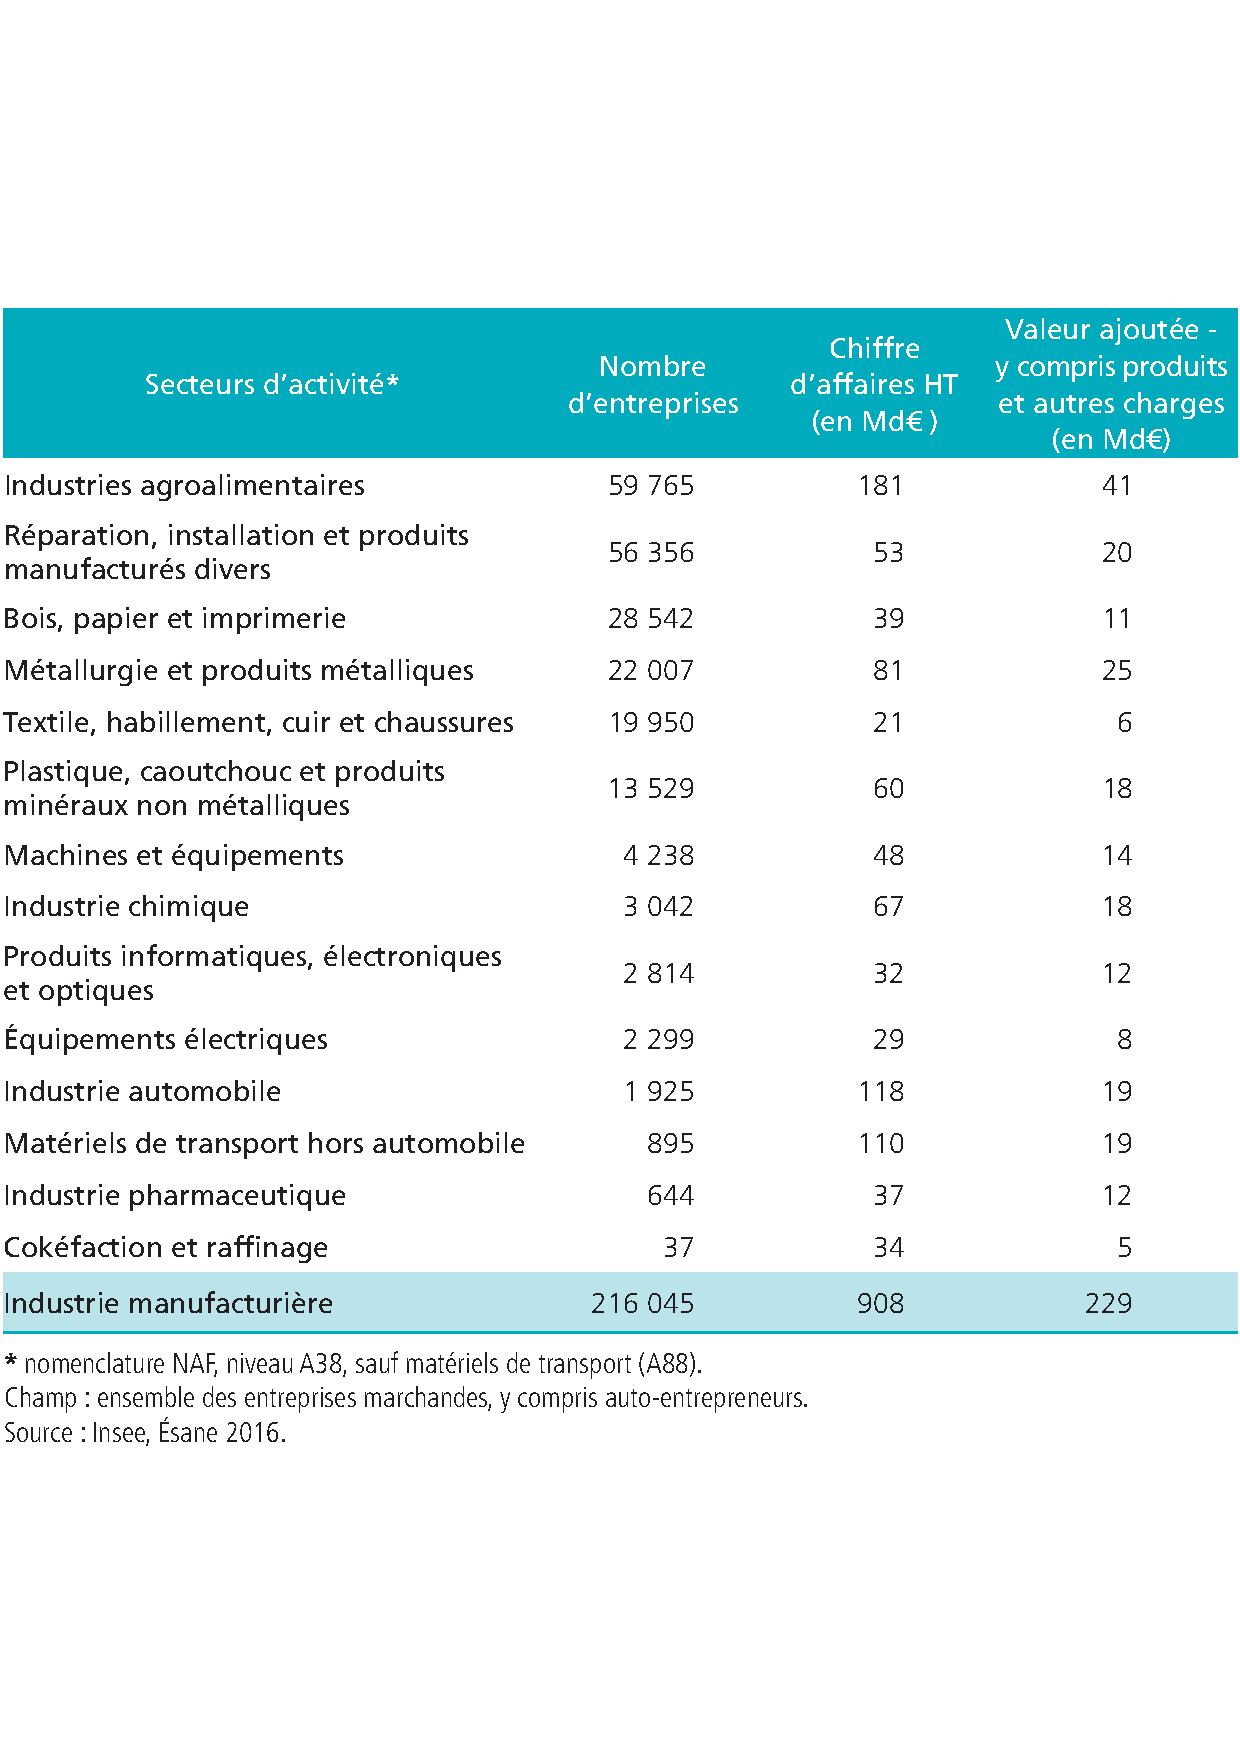
\includegraphics[width=\textwidth,height=\textheight,keepaspectratio]{../Chap1/Figures/2018-Chiffres-cles-industrie-manufacturiere-secteur.pdf}
	\caption{Figure issue du rapport annuel de la \citeauthor{directiongeneraledesentreprises_chiffres_2019} :  \citetitle{directiongeneraledesentreprises_chiffres_2019} \cite{directiongeneraledesentreprises_chiffres_2019}}
	\label{tab:state_art_compare}
\end{figure}

Contrairement à la transformation de la matière première, le contrôle de la qualité n'apporte pas de valeur au produit final ; c'est une sécurité pour respecter le cahier des charges et palier aux dérives du procédé.
C'est pourquoi le coût d'intégration d'un dispositif de mesure de la qualité se doit d'être faible.

Le contrôle qualité à cent pour-cent présente un coût d'installation et de fonctionnement.
Il est nécessaire de définir les caractéristiques d'un système de mesure économiquement viable, pour les productions industrielles.

\subsubsection{Intérêt économique du contrôle de la qualité en ligne de production}
% Aller capter des infos qui sont porteuses de l'info de non-conformité mais qui ne sont pas directement la conformité finale.
% 7.2.1	Maitrise Statistique du Procédé (MSP/SPC)
% Les variations brutales peuvent être détectées par une analyse MSP/SPC des variables-machine en temps réel, mais les dérives faibles et lentes sont difficilement détectées.
% L’objectif de toute surveillance SPC est de détecter ces dérives le plus tôt possible pour éviter de produire. 
La mesure par prélèvement de pièces, sur un procédé qui possède des étapes successives, ne permet pas d’identifier l’étape à l’origine du défaut.
Pour un produit qui nécessite un niveau de qualité élevé, un contrôle qualité final de chaque pièce sera réalisé (contrôle à cent pour-cent).
Dans le cas de l'injection-moulage de pièces plastiques, le contrôle qualité final est effectué bien après l’étape de moulage.
Le contrôle final est réalisé après l’ajout de valeur des étapes de finitions, ce qui prend parfois plusieurs jours.
Si la pièce était de mauvaise qualité juste après le moulage, alors de la valeur a été ajoutée à une pièce mauvaise.
Ce coût peut être très important pour une production industrielle.
Les coûts des étapes de finitions, telles que la peinture ou la galvanoplastie, sont bien plus importants que le coût de l'injection-moulage.
Le temps de cycle du procédé permet de produire une pièce toutes les 30 secondes, ce qui correspond pour une journée à milles pièces.
Si le défaut de qualité est détecté un jour après son apparition, cela correspond à 1000 pièces rebuts qui ont été finit inutilement.
L’objectif du contrôle qualité en ligne est de détecter les dérives de la qualité le plus tôt possible, afin d'éviter de produire.
Dans un second temps, il pourrait être possible d'ajuster les paramètres du procédé pour corriger les dérives qualité.

\subsubsection{Coût acceptable du dispositif de mesure}
% 2.1 Viabilité économique de la possession du dispositif de mesure
Dans le cas de l’injection plastique, le coût de la matière première et de l’étape d’injection-moulage est très faible en comparaison du coût des étapes de finitions. Produire des pièces mauvaises à un coût négligeable en comparaison du coût des étapes de peinture et de finitions de pièces mauvaises.
Détecter les pièces mauvaises dès la sortie de la presse d’injection, afin de les écarter de la chaîne de production, permet de diminuer les rebuts finaux et de supprimer ainsi les coûts associés à leurs finitions.
Le coût économique du dispositif de mesure est à rapporter au coût économique des rebuts.
Des industriels nous ont confirmés que le coût de la production de rebuts est faible en comparaison du coût de déploiement d’un dispositif de mesure sur chaque machine.
Si le coût du système de mesure dépasse la dizaine de milliers d’euros, il n’est pas intéressant.
Un coût élevé restera néanmoins intéressant à plus long terme, or nous cherchons à obtenir une adoption rapide.

La méthode la plus utilisée afin de maitriser le procédé d'injection-moulage est de positionner des capteurs à l’intérieur de l'outillage, directement en contact avec la matière.
Une analyse multi-variée permet ensuite de détecter les dérives du procédé.
Les capteurs les plus répandus sont les sondes de températures et les sondes de pressions \cite{kurt_experimental_2009}.
% Les données de ces capteurs sont analysées par différentes méthodes non-supervisés (carte de contrôle [Min, 2003], Analyse en Composante Principale [Zhang et al., 2015]) afin de détecter les dérives qualité sur une production stabilisée. La construction de modèle par apprentissage supervisé a également été proposée [Zhou et al., 2018]. Des capteurs plus complexes [Chen et al., 2004] et multivariés [Kazmer et al., 2011] ont été proposés, puis validés [Gordon et al., 2017].
Le coût de l’instrumentation invasive des moules est élevé.
D’après nos chiffrages régionaux, l’intégration de capteurs dans l'outillage représente un surcoût de vingt pour-cent de la conception et de la fabrication de l'outillage, pour un coût initialement compris entre cinquante et cent mille euros.
Intégrer les conduits nécessaires au passage des fils et connecteurs est compliqué sachant que les moules intègrent également des canaux de refroidissements indispensables au procédé.
Les capteurs subissent de fortes contraintes ce qui peut limiter leur durée de vie.
% Mais nous avons surtout observé des défaillances dans les fils de connections, lors des manipulations des moules pour les changements de productions.
Enfin, un capteur intégré à un outillage est associé un outillage, et donc à une unique pièce.
Il n'est pas viable de démonter l'instrumentation du capteur pour le positionner sur un autre outillage.
À contrario, un dispositif de mesure extérieur au procédé ne serait pas lié à un outillage.
Cela permettrait de contrôler la qualité quand le cahier des charges le nécessite, quel que soit la pièce produite.
L'installation du dispositif de mesure devra être simple, d'une durée inférieure à une heure, pour que sa mobilité soit réelle.
Un tel dispositif de mesure s'inscrit dans la démarche de l'industrie agile, où les lignes de productions sont fréquemment reconfigurées, en fonction des besoins.


\subsection{Faisabilité technologique de la mesure de la qualité en ligne de production}
Pour identifier un procédé, il est nécessaire de réaliser des mesures afin de connaître l'état de celui-ci à différents instants discrets.
Afin de pouvoir analyser l'évolution du procédé, l'échantillonnage des mesures doit être supérieure au temps caractéristique d'évolution du procédé.
Dans le cas de l'injection-moulage, la périodicité court-terme du procédé est celle du cycle de production d'une pièce, soit le temps de cycle du procédé, de 10 à 60 secondes.

% Aller capter des infos qui sont porteuses de l'info de non-conformité mais qui ne sont pas
Pour respecter cette contrainte, nous distinguons deux grands types de mesures :
\begin{itemize}
\item les mesures dites "invasives", qui nécessite l'installation de capteurs de grandeurs physiques à l'intérieur de l'outillage,
\item les mesures "non-invasives", qui s'intéressent à la pièce produite dès qu'elle sort de l'outillage.
\end{itemize}

% Les capteurs dans le moule peuvent mesurer la pression, la température ou bien la vitesse de déplacement de la matière par effet Doppler.
% En 2019, les systèmes d'acquisition utilisés avec ces capteurs fonctionnent à une fréquence de 25 à 1000 Hertz.
% Ainsi, le nombre de valeurs discrètes mesurées pendant un cycle est de l'ordre de dix milles.

Les mesures "invasives" nécessitent un travail de conception de l'outillage compliqué.
L'outillage intègre des canaux de refroidissement et le câblage des capteurs doit être conçu pour les éviter.
C'est pourquoi, \citeauthor{gao_multivariate_2012} proposent un capteur qui communiquent sans connectivité filaire \cite{kazmer_feasibility_2011, gao_multivariate_2012}.
L'outillage en acier conducteur est une cage de Faraday idéale.
La communication radiofréquence  est impossible.
C'est pourquoi ce capteur utilise des ondes acoustiques pour communiquer.
L'alimentation en énergie est assurée par le capteur, en récupérant les variations de pressions créées lors du cycle l'injection.
Cependant, cette solution n'est pour l'instant pas commercialisée.
De plus, la maintenance des capteurs intégrés à l'outillage est compliquée.
Les capteurs sont fragiles et les contraintes physiques qui s'exercent sur eux lors du cycle d'injection sont élevées.
En particulier, nous avons observé que les défaillances proviennent le plus souvent des câbles et non des capteurs eux-mêmes.
En cas de défaillance d'un capteur, c'est l'ensemble de l'outillage qui est immobilisé, ce qui impacte fortement la production industrielle.
À contrario, la mesure des pièces, dès leur sortie de l'outillage, ne demande pas ce travail de conception avancée.
Le système de mesure est éloignée des contraintes physiques du procédé d'injection-moulage, ce qui limite le besoin de maintenance.
% Un système de mesure avec des imageurs est positionné en sortie de moule afin de mesurer la pièce.
% L'objet de ces travaux de thèse est le développement d'un système de mesure non invasif de la qualité des pièces produites.
% Cette démarche s'inscrit dans une réduction des coûts de l'instrumentation des moules et dans une logique de mesure directe de la qualité géométrique et d'aspect visuel de la pièce au plus tôt dans la chaîne de production.

Pour être intégrée à la ligne de production, la mesure doit être réalisée dans une durée inférieure au temps de cycle du procédé d'injection-moulage.
Cette contrainte permet de réaliser le contrôle de cent pour-cent des pièces.
Si la pièce doit être déplacée devant le moyen de mesure, la durée du convoyage doit également être inclue.
De plus, si un ajustement des paramètres du procédé est attendu dès la pièce suivante, il est alors nécessaire d'effectuer l'analyse de la mesure pendant le temps de cycle.
Ces contraintes réduisent d'autant plus la durée disponible pour réaliser la mesure.
Nous estimons la durée maximale de la mesure à 10 secondes.
La Figure \ref{fig:time_constraint} inscrit la mesure dans le chronogramme du cycle du procédé (§\ref{fig:chronogramme}).
Cette limite sera une contrainte forte pour l'ensemble des choix technologiques de nos travaux.

\begin{figure}[hbtp]
	\centering
	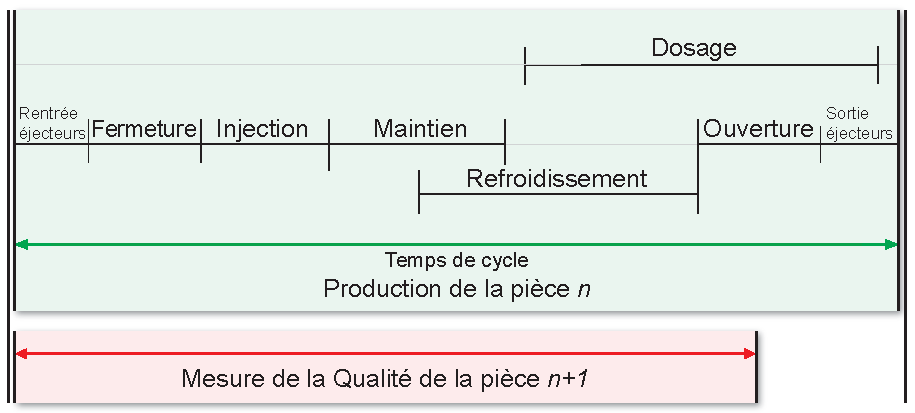
\includegraphics[width=\textwidth,height=\textheight,keepaspectratio]{../Chap1/Figures/SAPRISTI_Chronogramme-Simple.pdf}
	\caption{Intégration de la mesure dans le cycle d'injection-moulage.}
	\label{fig:time_constraint}
\end{figure}

Différentes mesures sont aujourd'hui compatibles, de par leurs courtes durées, avec une utilisation en cycle industriel : pesée de la masse, imagerie par thermographie infrarouge, contrôle d'aspect par caméras, imagerie tridimensionnelle \cite{schwenke_optical_2002}, durométrie, imagerie des champs de contraintes par l'imagerie des phénomènes de photoélasticité sur les pièces plastiques transparentes.
Pour obtenir des mesures fiables et répétables la mesure doit être automatisée.
C'est un des objectifs de nos travaux.
Nous discuterons de manière approfondie des techniques de mesure existantes dans le Chapitre \ref{ch:measure}.

\subsection{Formalisation de la notion de qualité et intégration de l'expert humain}
Aucune norme ne statue actuellement sur la qualité d'aspect.
Plusieurs travaux de recherches sont en cours.
On distinguera la sensation tactile \cite{bruno_albert_formalisation_2016, albert_generic_2016, albert_smart_2017, albert_smart_2019, albert_maitrise_2019} de l'aspect esthétique \cite{desage_syntactic_2015}.
Ces travaux associent une démarche de spécifications de la qualité, aux développements de nouveaux moyens de mesures \cite{desage_constraints_2015, pitard_metrologie_2016, lacombe_exploitation_2018a}.
Nos travaux s'inscrivent dans cette démarche de recherche.

Les pièces produites en injection-moulage des thermoplastiques possèdent une grande variété de dimension, de forme et d'état de surface.
Au sein d'une même entreprise, un système de contrôle de la qualité doit être capable de mesurer une grande variété de pièces.
Nous chercherons à simplifier au maximum l'utilisation de notre système de mesure afin de maximiser son adoption, tout en répondant à la problématique du contrôle de la qualité en ligne de production.

Le principal objectif est d'exploiter l'information issues des capteurs, afin de proposer une mesure de la qualité d'aspect.
La qualité d'aspect est une notion subjective qui est souvent définie dans les cahiers des charges sous la forme de défauthèques.
L'interprétation de ces définitions nécessite le travail d'un expert qualité humain.
L'expert qualité est généralement le référent de la notion de qualité pour un atelier de production.
Il forme les opérateurs, afin de leur transmettre les exigences qui sont interprétées à partir du cahier des charges.
Malheureusement, la transmission du savoir et la répétabilité de la mesure de la qualité par différents opérateurs, sont difficiles à mettre en œuvre.
Dans nos travaux, nous chercherons à automatiser cette interprétation.
Le système réalisera l'interprétation des mesures à partir d'un modèle de la qualité construit par apprentissage (Chapitre \ref{ch:metric_learning}).
À terme, l'objectif est de proposer un modèle de la qualité qui serait générique à tous types de pièces, ; tel qu'un humain formé à l'expertise qualité est capable d'inspecter tous types de pièces.

% \subsection{Apprentissage statistique pour l'exploitation des mesures}
% L'exploitation des mesures multi-modales par un humain est compliqué.
% De plus, il est nécessaire d'adapter le système pour chaque pièce.
% Nous cherchons à proposer un système générique à toutes pièces.
